%%%%%%%%%%%%%%%%%%%%%%%%%%%%%%%%%%%%%%%%%%%%%%%%%%%%%%%%%%%%%%%%%%%%%%%%%%%%%%%%%%%%
% IISER Thiruvananthapuram Presentation/Beamer Format
% LaTeX Template
%
% Author:
% Nikhil Alex Verghese, BS-MS 17, IISER Thiruvananthapuram
% PLEASE FORWARD ANY AND ALL SUGGESTIONS AND COMPLAINTS TO: nikhil.alexv17@alumni.iisertvm.ac.in
%
% READ ALL INSTRUCTIONS (presented as comments) IN EACH TEX FILE CAREFULLY.
%
% License:
% CC BY-NC-SA 4.0 (http://creativecommons.org/licenses/by-nc-sa/4.0/)
%
%%%%%%%%%%%%%%%%%%%%%%%%%%%%%%%%%%%%%%%%%%%%%%%%%%%%%%%%%%%%%%%%%%%%%%%%%%%%%%%%%%%%

% Refer to these super useful links for beamer tips and tricks
% http://tug.ctan.org/macros/latex/contrib/beamer/doc/beameruserguide.pdf
% https://www.overleaf.com/learn/latex/Beamer

%-----------------------------------------------------------------------------------
%	PACKAGES AND OTHER DOCUMENT CONFIGURATIONS
%-----------------------------------------------------------------------------------

\documentclass[10pt,presentation,shownotes]{beamer}
\usetheme{Warsaw}
\usecolortheme{crane} % Yellow and Blue color scheme
\usepackage{beamerthemesplit}
\usefonttheme{default}
\setbeamertemplate{caption}[numbered]
\setbeamercolor{block body example}{bg=green!12}
\setbeamertemplate{navigation symbols}{} % Uncomment to disable the bottom right navigation buttons
\setbeamercovered{transparent}
\setbeamertemplate{theorems}[numbered]
% THE FOLLOWING TEMPLATE IS FRAGILE: It is recommended you familiarise yourself with 
% a rough idea of the presentation's framework before adding custom elements.

\usepackage[utf8]{inputenc}
\usepackage[T1]{fontenc}
\usepackage{lmodern}
\usepackage[spanish]{babel}
\usepackage{csquotes}
\usepackage{mathtools,amsfonts,amssymb,setspace}

\usepackage{pstricks} % PSTricks offers an extensive collection of quick and easy macros for generating PostScript including macros for colour, graphics, pie charts, rotation, trees and overlays.
% (https://ctan.org/pkg/pstricks-base?lang=en)

\usepackage{hyperref} % hypperref package for creating reliable hyperlinks and customizations
% (https://ctan.org/pkg/hypperref?lang=en)

\usepackage{tikz} % Tikz package for drawing graphs and diagrams [XY-pic is now outdated]
% (https://ctan.org/pkg/tikz?lang=en, https://www.overleaf.com/learn/latex/TikZ_package)

%\usepackage{tikz-cd} % Commutative Diagrams with Tikz, primarily for linear algebra.
% (https://ctan.org/pkg/tikz-cd?lang=en)

%\usepackage{pgfplots} % The Pgfplots package is dependent on tikz package and is used to portray
% detailed 2D and 3D function plots from scratch as well as plot available data with a high degree
% of customization (https://www.overleaf.com/learn/latex/Pgfplots_package) 
% (https://ctan.org/pkg/pgfplots?lang=en)

%\usepackage{caption} % The captions package allows you to better control captions for floating environments like figures, etc. (https://ctan.org/pkg/caption?lang=en)

%\usepackage{booktabs} % The booktabs package allows better control over tables including ruling, width, etc. (https://ctan.org/pkg/booktabs?lang=en) 

\usepackage{booktabs}
\usepackage{multirow}
\usepackage{graphicx}
\usepackage{xcolor} % Customize colours for hyperlinks, etc.
% (https://ctan.org/pkg/xcolor?lang=en)
\hypersetup{
	colorlinks,
	linkcolor={blue!50!black},
	citecolor={blue!50!black},
	urlcolor={blue!80!black}
}

\usepackage{appendixnumberbeamer} % This resets the page count after the \appendix function is called, unlike the traditional appendix package (https://ctan.org/pkg/appendixnumberbeamer?lang=en)

\usepackage[backend=biber,style=alphabetic]{biblatex} % We use BiBLaTeX for our bibliography.
% (https://ctan.org/pkg/biblatex?lang=en)
\renewcommand*{\nameyeardelim}{\addcomma\addspace}
\addbibresource{References/ref.bib}

% The lipsum package called in the next line is just for generating dummy text throughout this template and is not necessary.
\usepackage{lipsum}

% Note: Changes to specific presentation elements usually start with /makeatletter and ends with /makeatother

% Defining an Example Block
\makeatletter
\def\th@remark{%
    \normalfont % body font
    \setbeamercolor{block title example}{bg=orange,fg=black}
    \setbeamercolor{block body example}{bg=orange!20,fg=black}
    \def\inserttheoremblockenv{exampleblock}
  }
\makeatother

\theoremstyle{remark}
\newtheorem*{remark}{Remark}

% Setting Header Properties
\setbeamertemplate{headline}
{
  \leavevmode%
  \hbox{%
  \begin{beamercolorbox}[wd=.5\paperwidth,ht=2.5ex,dp=1ex,left,leftskip=1em]{section in head/foot}%
    \usebeamerfont{subsection in head/foot}\hspace*{2ex}\insertshorttitle
  \end{beamercolorbox}%
  \begin{beamercolorbox}[wd=.5\paperwidth,ht=2.5ex,dp=1ex,center]{date in head/foot}%
    \usebeamerfont{date in head/foot}\insertshortdate{}\hspace*{2ex}
  \end{beamercolorbox}}%
  \vskip0pt%
}

% Setting Footer Properties
\makeatletter
\setbeamertemplate{footline}
{
  \leavevmode%
  \hbox{%
  \begin{beamercolorbox}[wd=.33\paperwidth,ht=2.25ex,dp=1ex,center]{author in head/foot}%
    \usebeamerfont{author in head/foot}\insertshortauthor~~\beamer@ifempty{\insertshortinstitute}{}{(\insertshortinstitute)}
  \end{beamercolorbox}%
  \begin{beamercolorbox}[wd=.34\paperwidth,ht=2.25ex,dp=1ex,center]{subsection in head/foot}%
    \usebeamerfont{section in head/foot}\hspace*{1ex}\insertsectionhead\hspace*{1ex}
  \end{beamercolorbox}%
  \begin{beamercolorbox}[wd=.33\paperwidth,ht=2.25ex,dp=1ex,right, rightskip=1em]{section in head/foot}%
    \usebeamerfont{section in head/foot}\insertsubsectionhead\hspace*{2ex}
  \end{beamercolorbox}}%
  \vskip0pt%
}
\makeatother

% Defining when a title is required for a frame
\makeatletter
\setbeamertemplate{frametitle}{
    \ifbeamercolorempty[bg]{frametitle}{}{\nointerlineskip}%
    \@tempdima=\textwidth%
    \advance\@tempdima by\beamer@leftmargin%
    \advance\@tempdima by\beamer@rightmargin%
    \begin{beamercolorbox}[sep=0.3cm,center,wd=\the\@tempdima]{frametitle}
        \usebeamerfont{frametitle}%
        \vbox{}\vskip-1ex%
        \if@tempswa\else\csname beamer@ftecenter\endcsname\fi%
        \strut\insertframetitle\strut\par%
        {%
            \ifx\insertframesubtitle\@empty%
            \else%
            {\usebeamerfont{framesubtitle}\usebeamercolor[fg]{framesubtitle}\insertframesubtitle\strut\par}%
            \fi
        }%
        \vskip-1ex%
        \if@tempswa\else\vskip-.3cm\fi% set inside beamercolorbox... evil here...
    \end{beamercolorbox}%
}
\makeatother

% This code displays a self-updating ToC at the beginning of every section.
\AtBeginSection[]
{
	\begin{frame}
	\frametitle{Flujo de la presentación}
	\tableofcontents[currentsection]
	\end{frame}
}

\makeatletter
\newcommand<>{\insertsubsectiontitle}{\frametitle{\insertsubsection}}
\let\oldbeamer@checkframetitle\beamer@checkframetitle% Store the \frametitle checking mechanism
\renewcommand<>{\subsection}{%
  \gdef\beamer@checkframetitle{% Update \frametitle checking to ...
    \insertsubsectiontitle% ...insert the section title and...
    \global\let\beamer@checkframetitle\oldbeamer@checkframetitle% ...revert to it's old definition
  }% Regular \section stuff follows
  \alt#1{\@ifnextchar[\beamer@subsection\beamer@@subsection}
    {\beamer@secgobble}}
\makeatother

% Defining proofs environment for proofs requiring more than one frame
\makeatletter
\newenvironment<>{proofs}[1][\proofname]{%
    \par
    \def\insertproofname{#1\@addpunct{.}}%
    \usebeamertemplate{proof begin}#2}
  {\usebeamertemplate{proof end}}
\makeatother

% Uncomment for some standard notations in math (Real, Complex and Rational numbers, Norm, Jacobian, etc) 
% \newcommand{\reals}{\mathbb{R}}
% \newcommand{\mtrx}{\mathbb{M}}
% \newcommand{\jacobian}{\mathcal{J}}
% \newcommand{\tallstrut}{\vphantom{\frac{5_A}{4,10^3}}}
% \newcommand{\abs}[1]{\left\lvert #1 \right\rvert}
% \newcommand{\norm}[1]{\left\lVert #1 \right\rVert}

%%%%%%%%%%%%%%%%%%%%%%%%%%%%%%%%%%%%%%%%%%%%%%%%%%%%%%%%%%%%%%%%%%%%%%%%%%%%%%
%                 TITLE PAGE, FILL IN FOR PLACEHOLDER TEXT                   %
%%%%%%%%%%%%%%%%%%%%%%%%%%%%%%%%%%%%%%%%%%%%%%%%%%%%%%%%%%%%%%%%%%%%%%%%%%%%%%

% Note: Longer input for Title Page, Abridged Input for Header and Footer

\title[\color{white}El papel del tamaño de los ciclones tropicales en la precipitación en México]{El papel del tamaño de los ciclones tropicales en la precipitación en México
}
\author[Adolfo Pérez]{Adolfo Pérez Estrada}
\institute[PCT UNAM]{Programa de Posgrado en Ciencias de la Tierra \\ Universidad Nacional Autónoma de México}
\date[\insertframenumber/\inserttotalframenumber]{Examen que opta por el grado de: \\ Maestro en Ciencias de la Tierra}
% (Major/Minor Project Presentation, Thesis Defense, etc.)
\titlegraphic{
\includegraphics[height=40pt]{Images/Logos/posgrado2.jpg}}

% Document starts here
\begin{document}

\setlength{\belowcaptionskip}{10pt plus 2pt minus 4pt}

% Title page
\begin{frame}[plain]
	\maketitle
\end{frame}

% Chapters
\section{Introducción}
\subsection{Los ciclones tropicales en México}
\begin{frame}
    \begin{figure}[H]
        \centering
        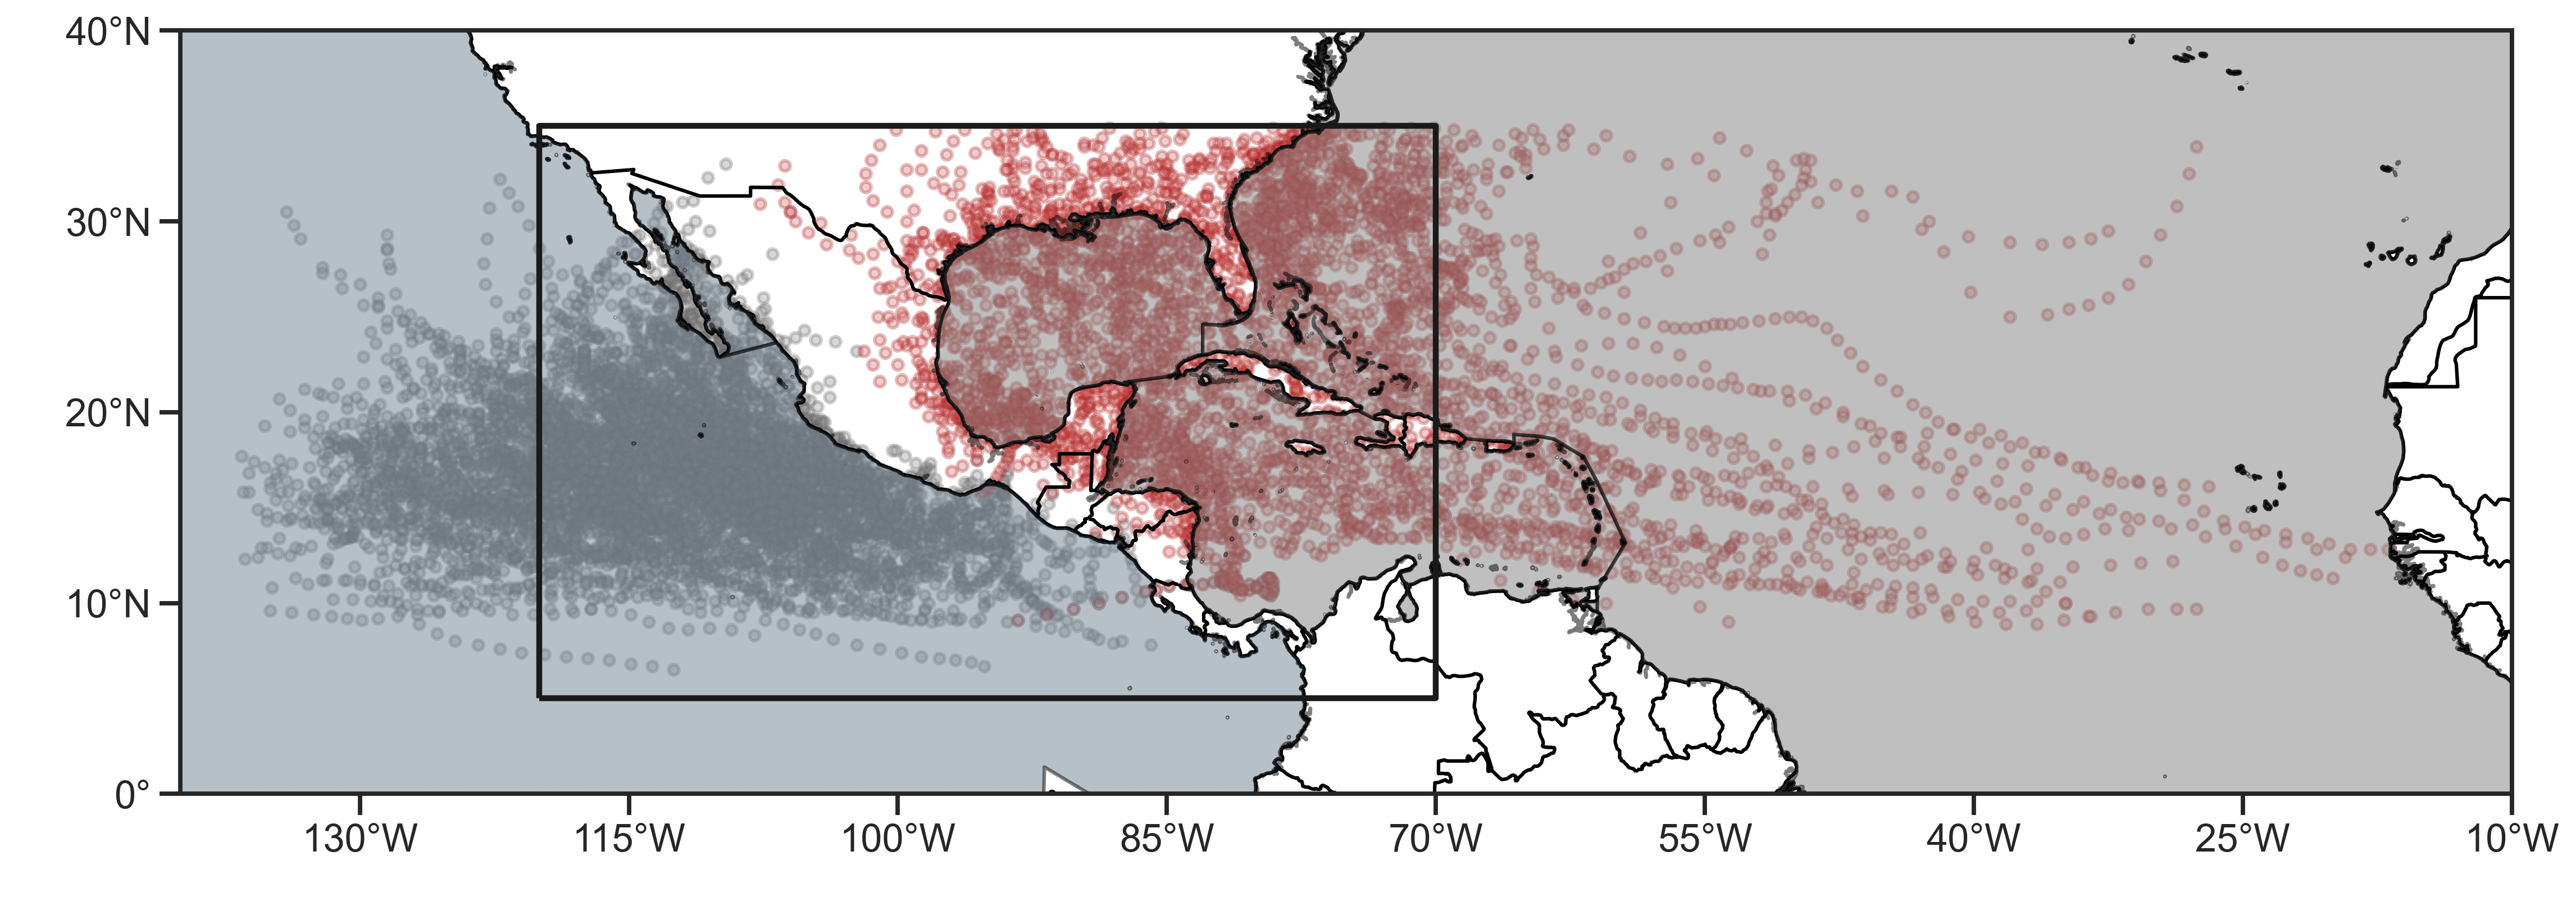
\includegraphics[scale = 0.275]{Images/Figures/Fig_2_1.jpeg}
        \caption{La región de estudio se encuentra marcada por un cuadro negro. Las posiciones de cada 6 horas de los CTs en el Océano Atlántico del norte (NA) y en el Océano Pacífico del este (EP) se encuentran en polígonos rojos y grises, respectivamente}
        \label{fig:fig_1}
    \end{figure}
\end{frame}

\begin{frame}{Escala Saffir-Simpson}
    % Please add the following required packages to your document preamble:

\begin{table}
\centering
\caption{Clasificación de los vientos de los CTs de acuerdo a la escala Saffir-Simpson. Se anexan dos categorías adicionales cuando el CT aún no alcanza la categoría de huracán (Kelman, 2013)}
\label{tab:1.1}
\resizebox{\textwidth}{!}{%
\begin{tabular}{@{}cccc@{}}
\toprule
\multicolumn{2}{c}{\textbf{Categoría}}               & \begin{tabular}[c]{@{}c@{}}\textbf{Vientos Sostenidos} \\ ($km  h^{-1}$)\end{tabular} & \begin{tabular}[c]{@{}c@{}} \textbf{Tipos de daño debido a}\\  \textbf{los vientos del CT}\end{tabular} \\ \midrule
\multicolumn{2}{l}{Depresión Tropical (DT)} & \textless 63                                                           & Daños menores                                                                             \\
\multicolumn{2}{l}{Tormenta Tropical  (TT)}  & 64-118                                                                 & Daños moderados                                                                           \\
\multirow{5}{*}{Huracán}         & 1        & 119-153                                                                & Vientos muy peligrosos                                                                    \\
                                 & 2        & 154-177                                                                & Vientos extremadamente peligrosos                                                         \\
                                 & 3        & 178-208                                                                & Daños devastadores                                                                        \\
                                 & 4        & 209-251                                                                & Daños catastróficos                                                                       \\
                                 & 5        & \textgreater 252                                                       & Daños extraordinarios                                                                     \\ \bottomrule
\end{tabular}%
}
\end{table}
\end{frame}

\begin{frame}
    \begin{figure}
        \centering
        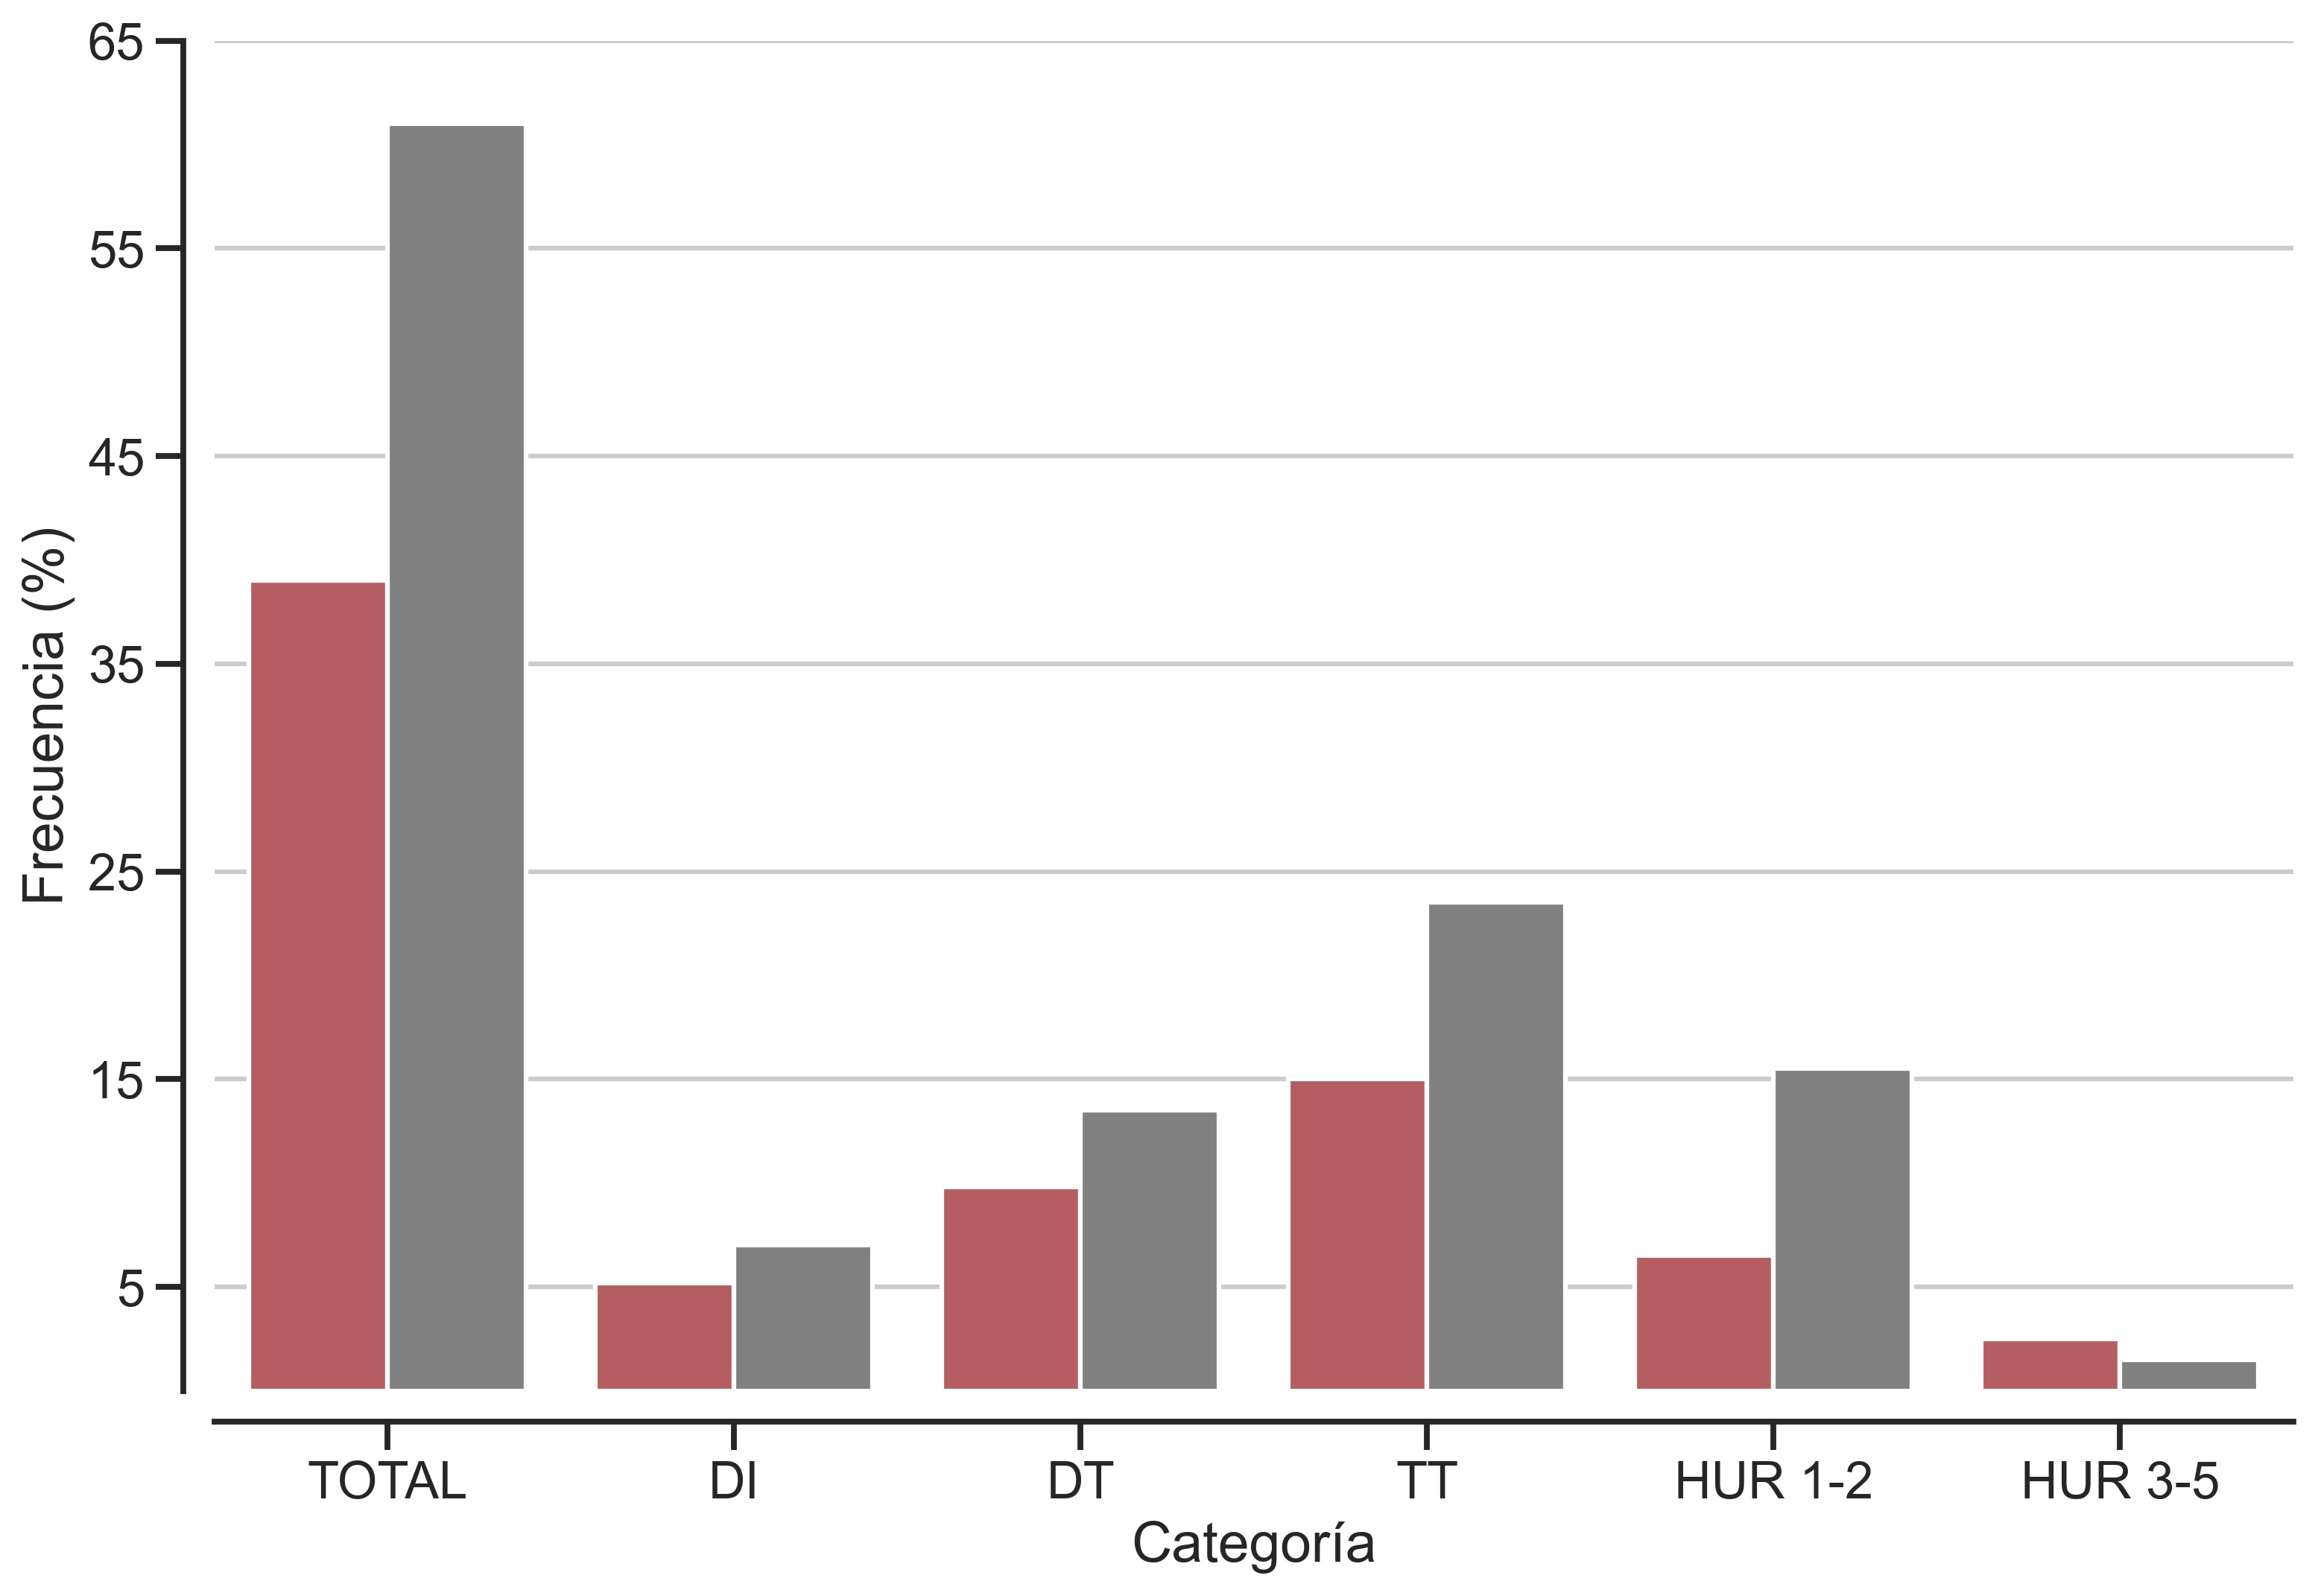
\includegraphics[scale=0.35]{Images/Figures/Fig_1_1.jpeg}
        \caption{Porcentaje de los CTs que hicieron \textit{landfalling} en las costas mexicanas. Los CTs del {\red NA} están en barras rojas  y los {\gray EP} en barras grises.}
        \label{fig:fig_2}
    \end{figure}
\end{frame}

\begin{frame}{El SIAT-CT en México}
    Los desastres históricos asociados al paso de CTs en México es la principal motivación para elaborar planes de acción y mejorar la gestión integral de riesgos. En el año 2000, se propone la creación de un Sistema de Alerta Temprana de Ciclones Tropicales (SIAT-CT) como una herramienta de coordinación entre la población y Protección Civil.

    \begin{block}{Peligro por CT definido por el SIAT-CT}
    \begin{equation}
    \label{eq:1.1}
       e = \displaystyle \frac{(I+C)}{2},
    \end{equation}
    
    $e = $ Peligro \\
    $I = $ Intensidad definida por la Escala Saffir-Simpson \\
    $C = $ Escala de circulación definido por el tamaño del radio de 34 nudos
    \\~\
    \end{block}
\end{frame}

\begin{frame}
\begin{columns}
    \begin{column}{0.35\textwidth}
        \begin{block}{SIAT-CT caso TT Cristobal}
        Representación del nivel de alerta del SIAT-CT para la TT Cristóbal el 4 de junio del 2020 en sus posiciones reportadas durante las 00:00(a), 06:00(b), 12:00(c), 18:00(d) y las 00:00(e) del 5 de junio.
        \end{block}
    \end{column}
    \begin{column}{0.65\textwidth}
    \begin{figure}
        \centering
        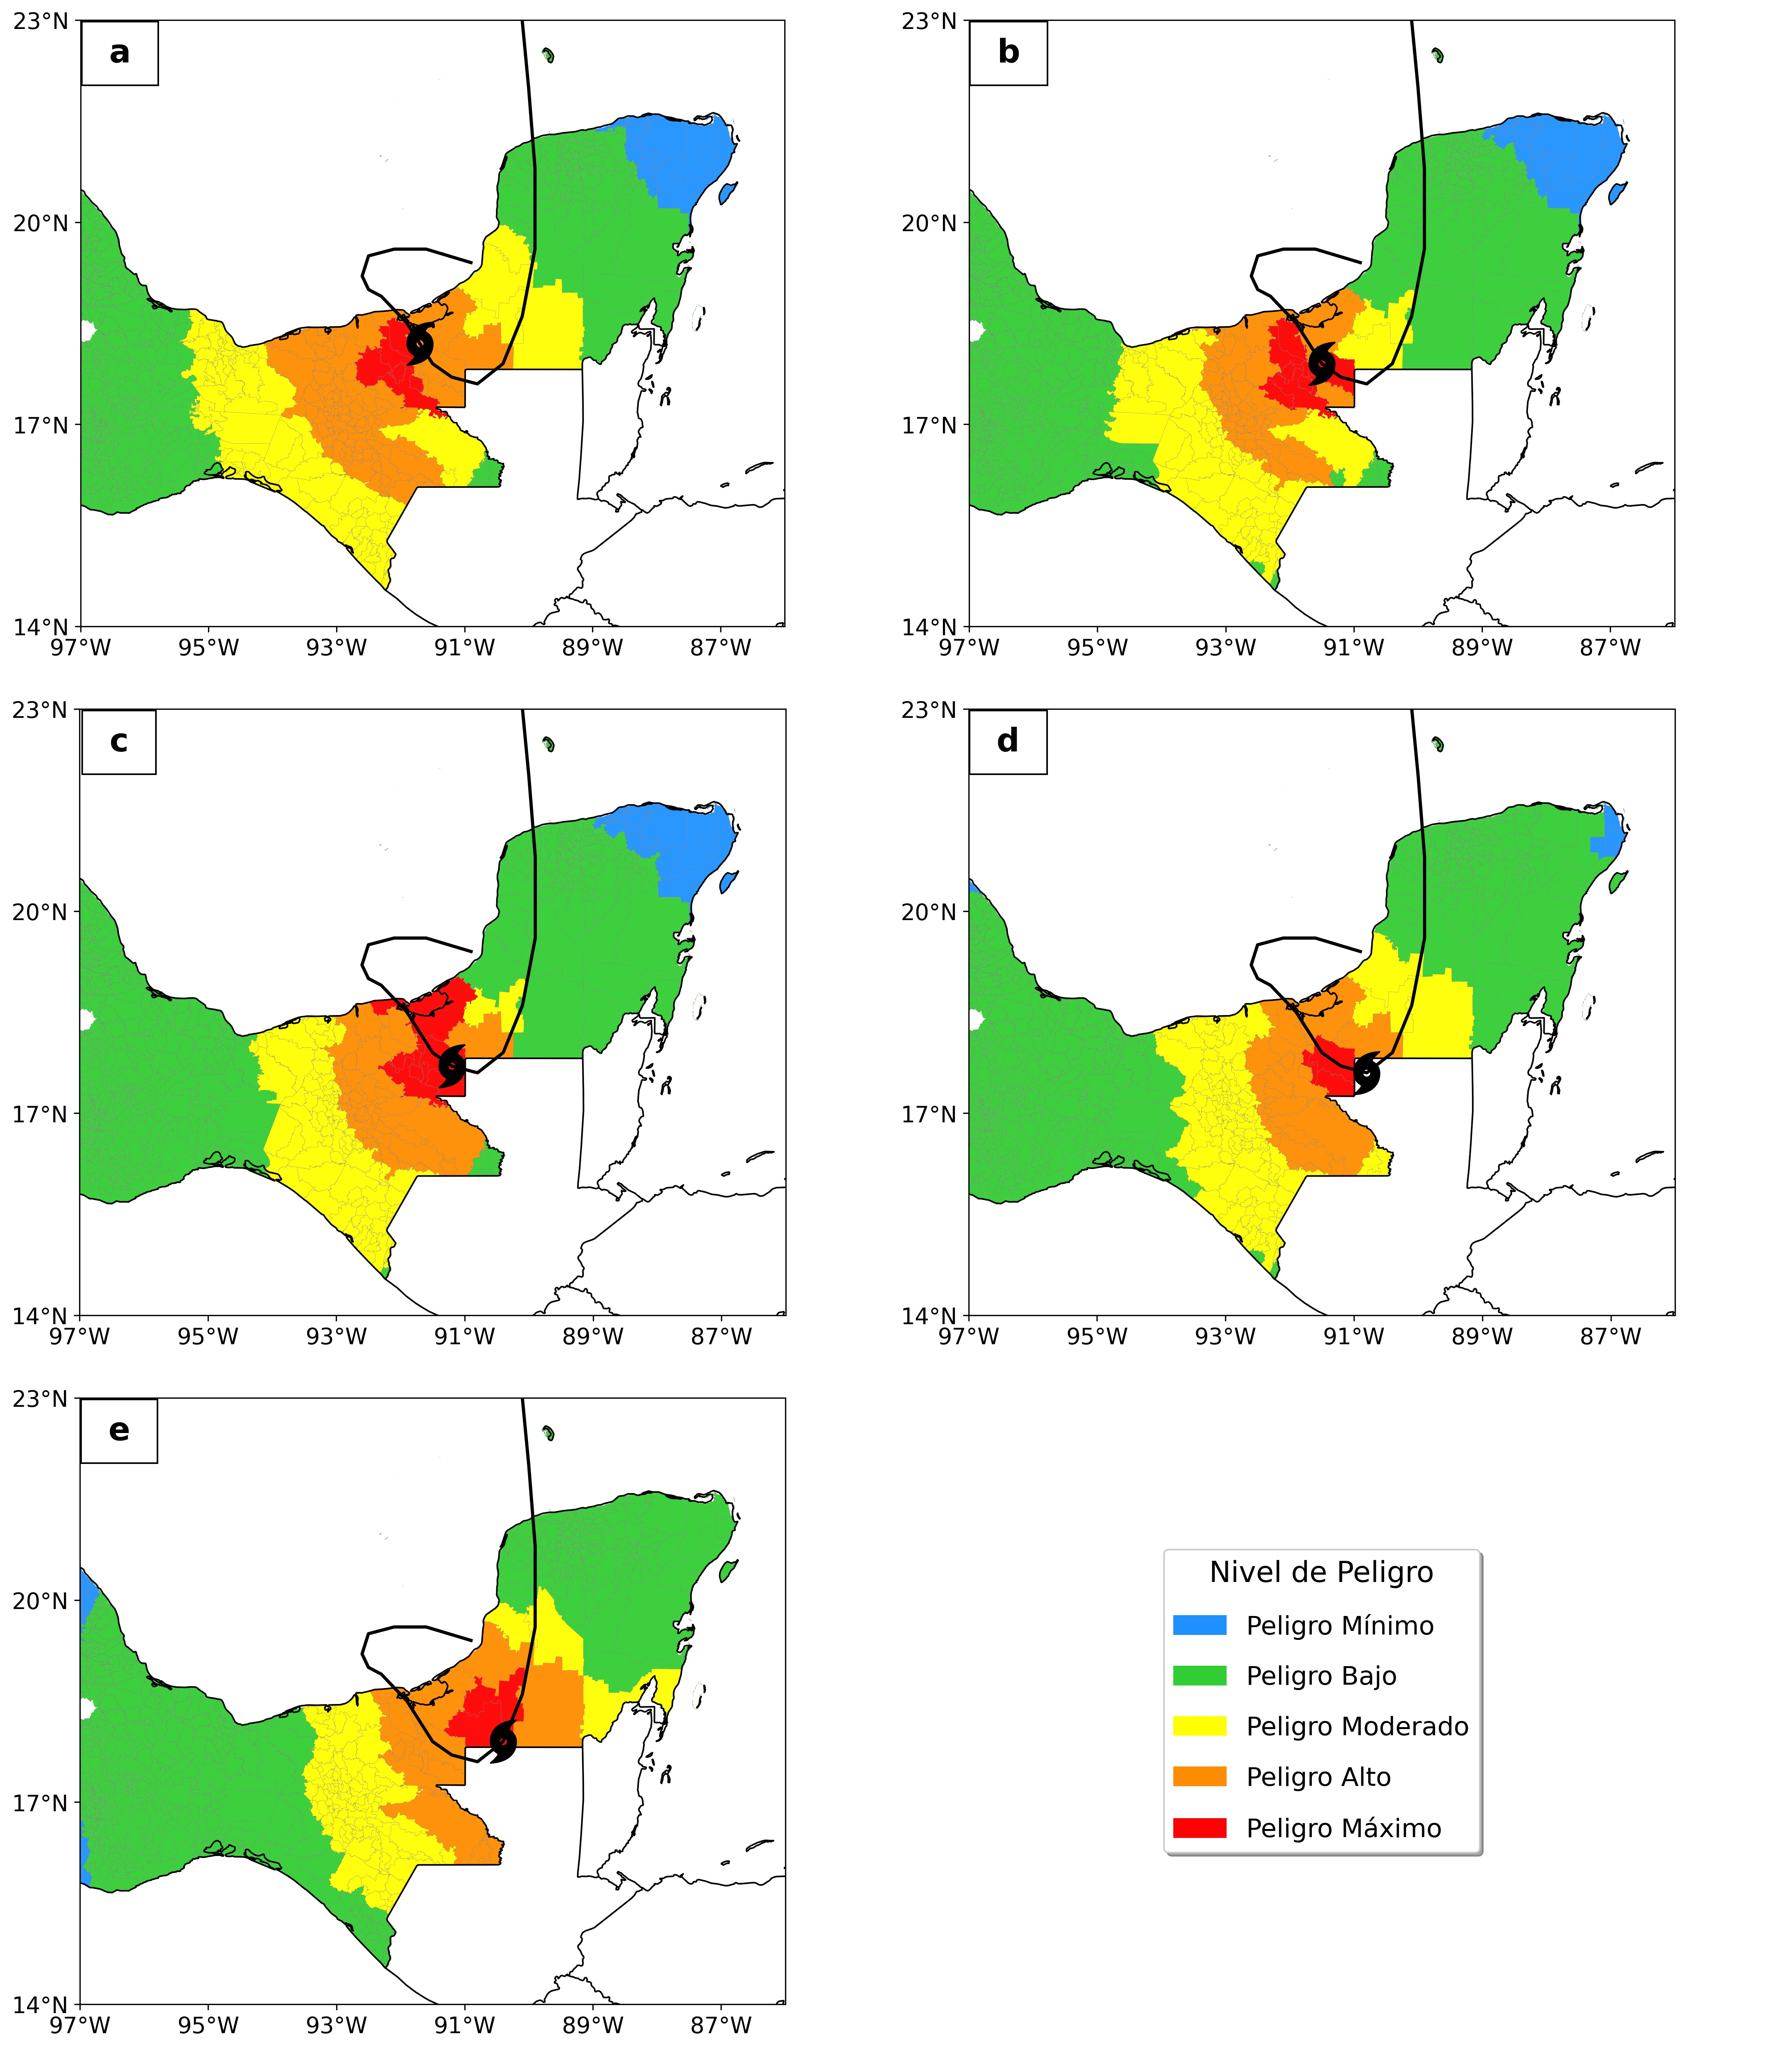
\includegraphics[scale = 0.18]{Images/Figures/Fig_1_3.jpeg}
        \label{fig:fig_3}
    \end{figure}
    \end{column}
\end{columns}
\end{frame}

\begin{frame}
    \begin{figure}
        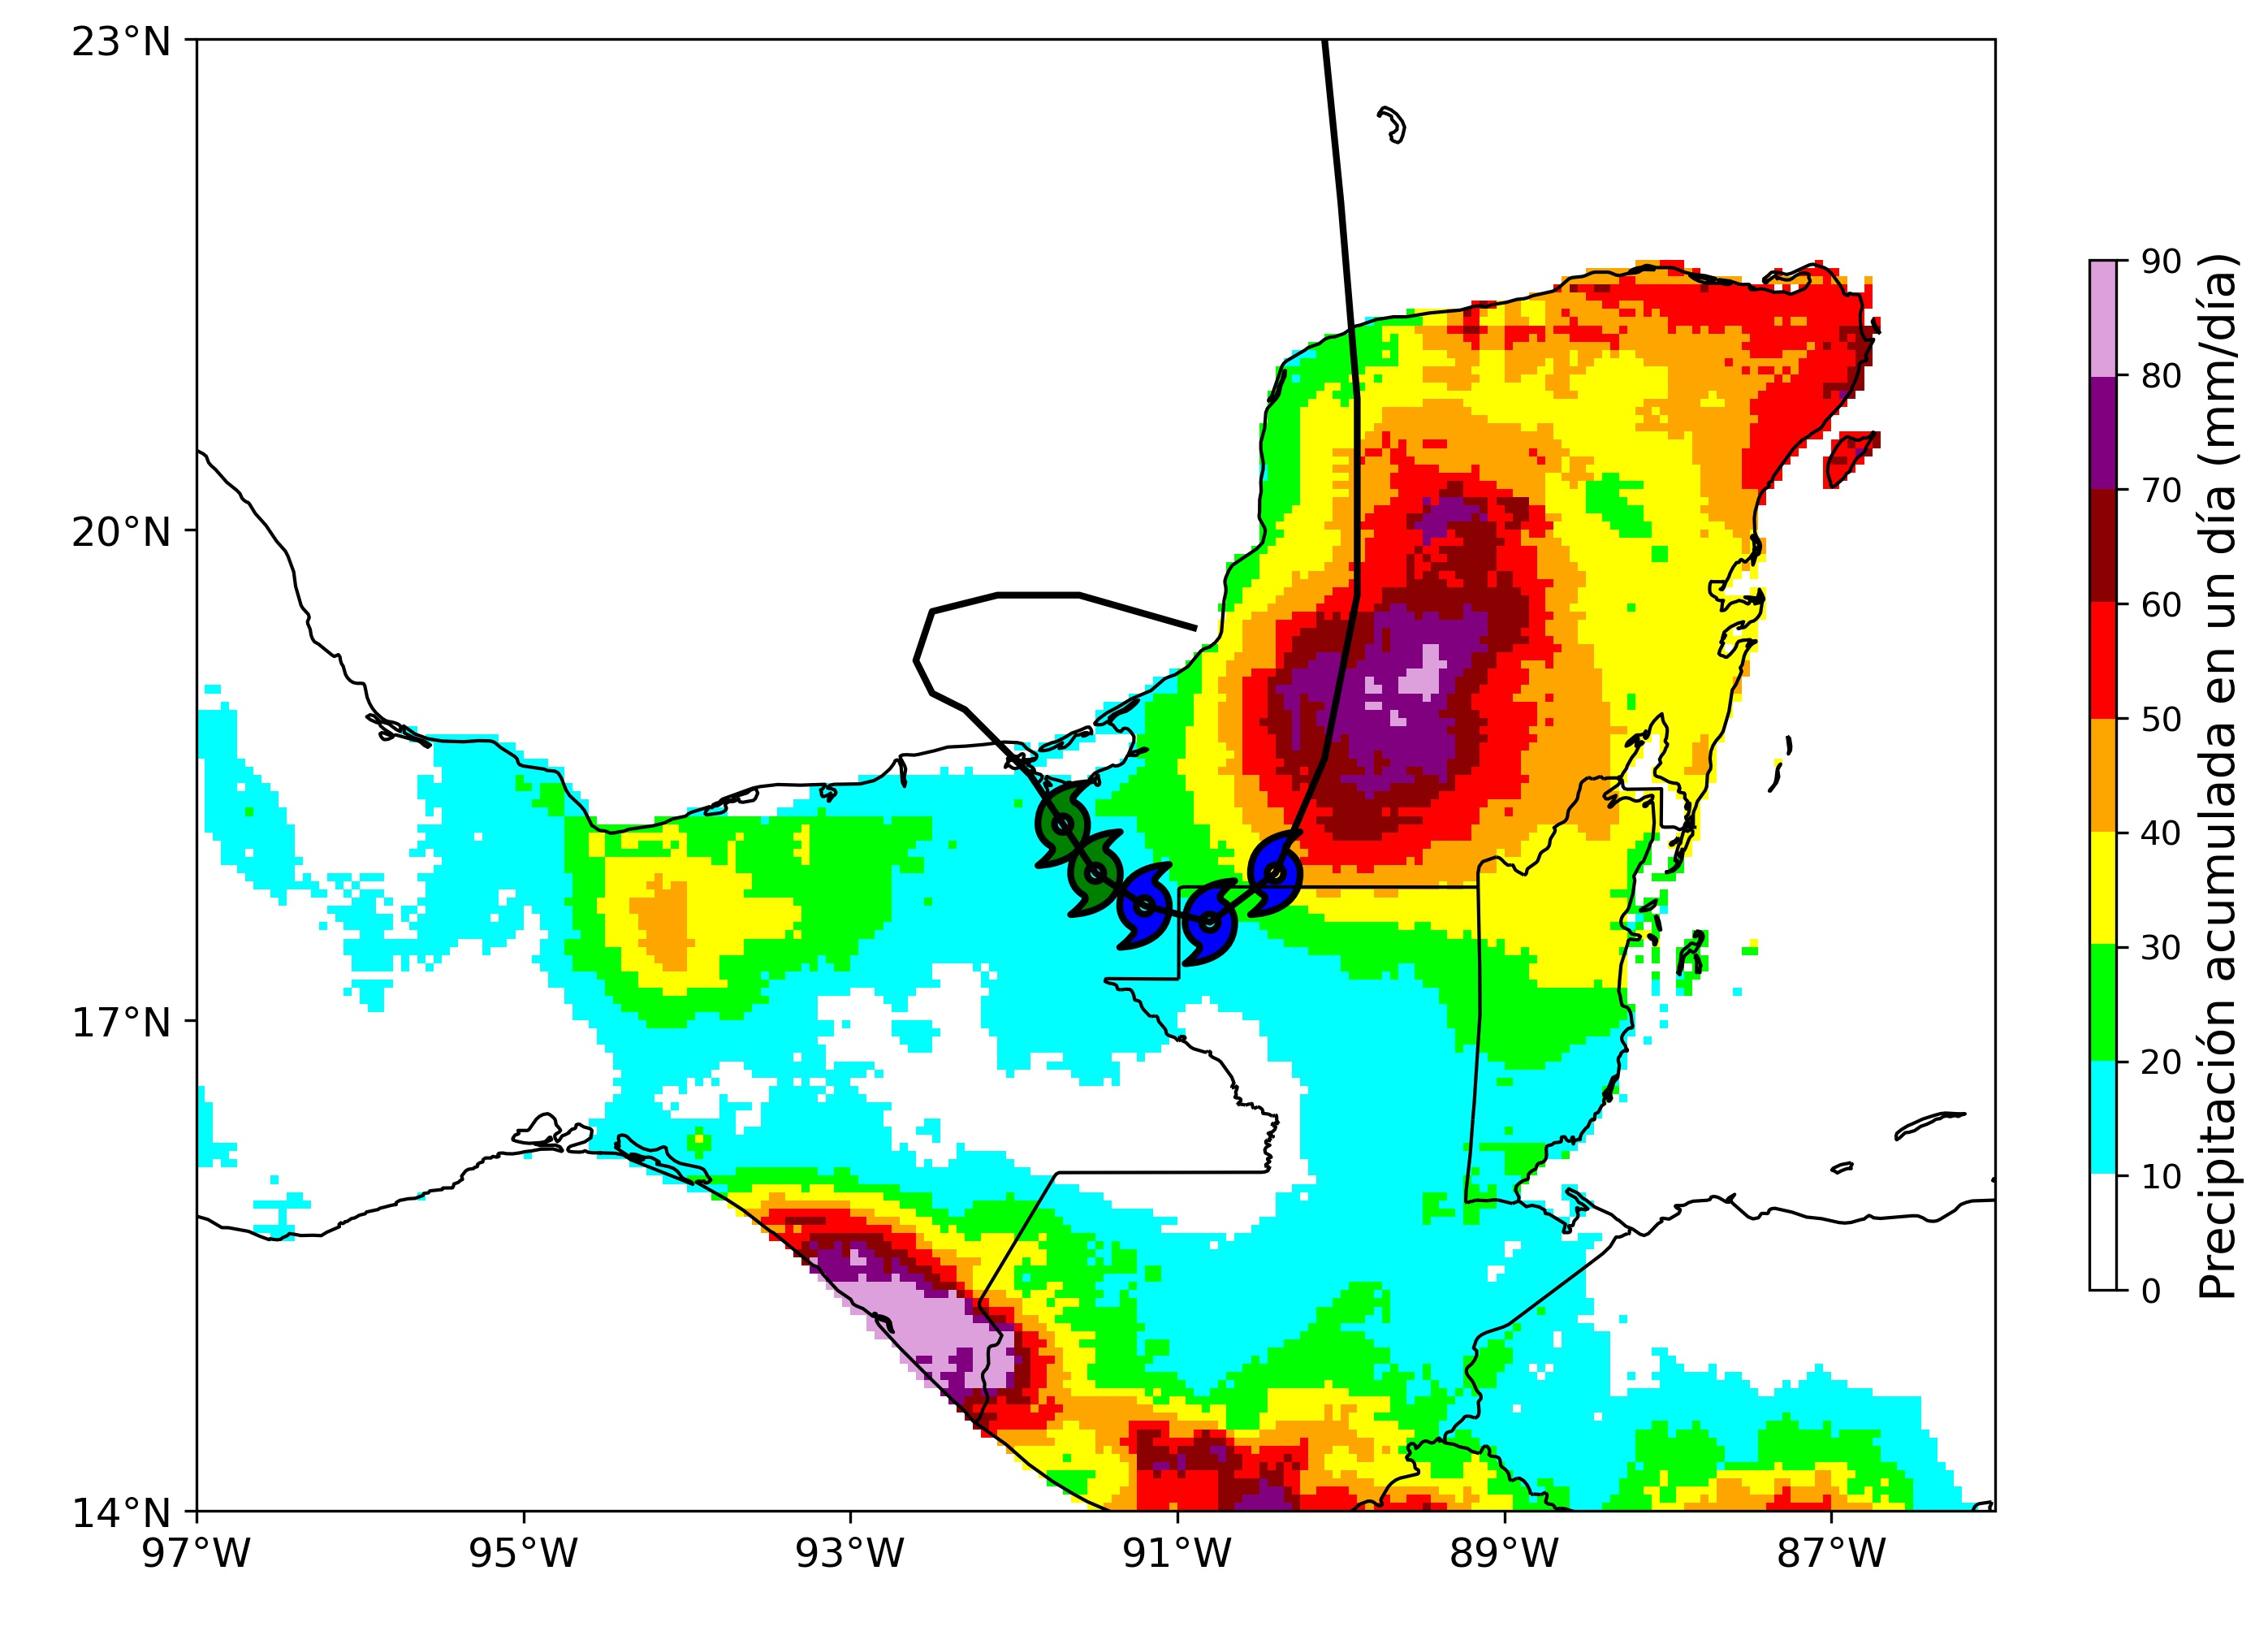
\includegraphics[scale = 0.35]{Images/Figures/Fig_1_2.jpeg}
        \caption{Valores de precipitación reportadas por CHIRPS el día 4 de junio del 2020 en el sureste de México. Las posiciones de la TT Cristóbal se muestran en verde (Tormenta Tropical) y azul (Depresión Tropical)}
        \label{fig:fig_4}  
    \end{figure}
\end{frame}

\subsection{Justificación y Objetivos}
\begin{frame}
    \hfill
    \begin{columns}
    \begin{column}{0.48\textwidth}
    \begin{block}{Justificación}
    Los estudios de CTs en México son limitados, aunque el país es impactado por la actividad ciclónica tropical cada año. Por ello, es necesario mejorar su definición de peligrosidad en el SIAT, con la finalidad de mejorar la gestión integral de riesgo. Es necesario contar con una metodología diseñada para México que defina el tamaño de los CTs.
\\~\ % Used for spacing out the block 
    \end{block}
    \end{column}
    \begin{column}{0.48\textwidth}
    \begin{block}{Objetivo General}
    Definir el tamaño de los ciclones tropicales que afectaron a México usando imágenes satelitales infrarrojas, así como analizar las relaciones estadísticas del tamaño con las variables medioambientales durante el periodo 2000-2020.
\\~\ % Used for spacing out the block 
    \end{block}
    \end{column}
    \end{columns}
\end{frame}

% \\~\ is used to force empty lines to generate to fix general typesetting within blocks.
% \\ = new line and ~\ = empty character
% \lipsum is used to generate dummy text.

\section{Datos y Métodos}

\begin{frame}{El tamaño del CT}
\textbf{¿Qué es el tamaño de los CTs?} \\ El término tamaño del CT suele ser muy ambiguo porque se puede abordar diferentes parametrizaciones considerando principalmente:
\begin{itemize}
    \item La velocidad del viento de los CTs
    \begin{itemize}
        \item Intensidad de los vientos en su circulación interna
        \item Intensidad de los vientos en su circulación externa
    \end{itemize}
    \item La vorticidad
    \item Isobaras (curva de igual o constante presión)
    \item Precipitación reportada a ciertos umbrales
\end{itemize}

\end{frame}

\subsection{Bases de datos utilizadas}
\begin{frame}
    \begin{block}{Para calcular el tamaño}
        \begin{itemize}
            \item Posiciones del CT cada 6 h HURDAT
            \item Productos IR del GPM
            \item Tamaño del campo de vientos.
        \end{itemize}
    \end{block}

    \begin{exampleblock}{Para validar relación entre el tamaño y precipitación}
        \begin{itemize}
            \item Producto satelital GPM\_IMERG
            \item Producto de precipitación CHIRPS
        \end{itemize}
    \end{exampleblock}

    \begin{alertblock}{Para la validación de las variables ambientales con la precipitación}
    Se utilizaron las siguientes variables: 
    Velocidad vertical del viento a 500 hPa, humedad específica a 600 hPa, vorticidad a 200 hPa, divergencia a 200 hPa, cizalladura del viento, contenido total de agua precipitable
    \end{alertblock}
\end{frame}

\subsection{ROCLOUD: Una nueva aproximación del tamaño del CT}
\begin{frame}
    \begin{block}{Sobre el tamaño de la circulación del CT}
        Pérez-Alarcón et al. (2021) desarrollaron una base de datos sobre el tamaño de los CTs utilizando los perfiles uniformes del viento descritos por Willoughby et al. (2006). \bigskip

        Estos cálculos utilizan la posición del CT obtenida del HURDAT2, la intensidad máxima de los vientos y el radio de los vientos máximos, calculado a través de modelos específicos para cada cuenca o en función de la posición latitudinal del CT.

    \begin{equation}
        \label{eq:2.1}
        r_{m} =  46.6 \ \exp{(-0.015 \ V_{max} + 0.0169 \phi)}
    \end{equation}
        \\~\
    \end{block}

\end{frame}

\begin{frame}
    Se diseñó un algoritmo que mide las distancias radiales desde el centro del CT hasta el punto más alejado donde las temperaturas de brillo de las nubes pertenecen a la circulación del CT y están por debajo de -40°C
    \\~\ 
    \\~\ 
\begin{enumerate}
    \item<1-> Segmentación a -40°C
     \\~\
    \item<2-> Selección de regiones de intéres
     \\~\
    \item<3-> Selección de poligonos dentro del campo de vientos
     \\~\
    \item<4-> Determinación de los radios por cuadrante
     \\~\
    \item<4-> Cálculo del radio promedio
\end{enumerate}
\end{frame}

\begin{frame}
    \begin{figure}
        \centering
        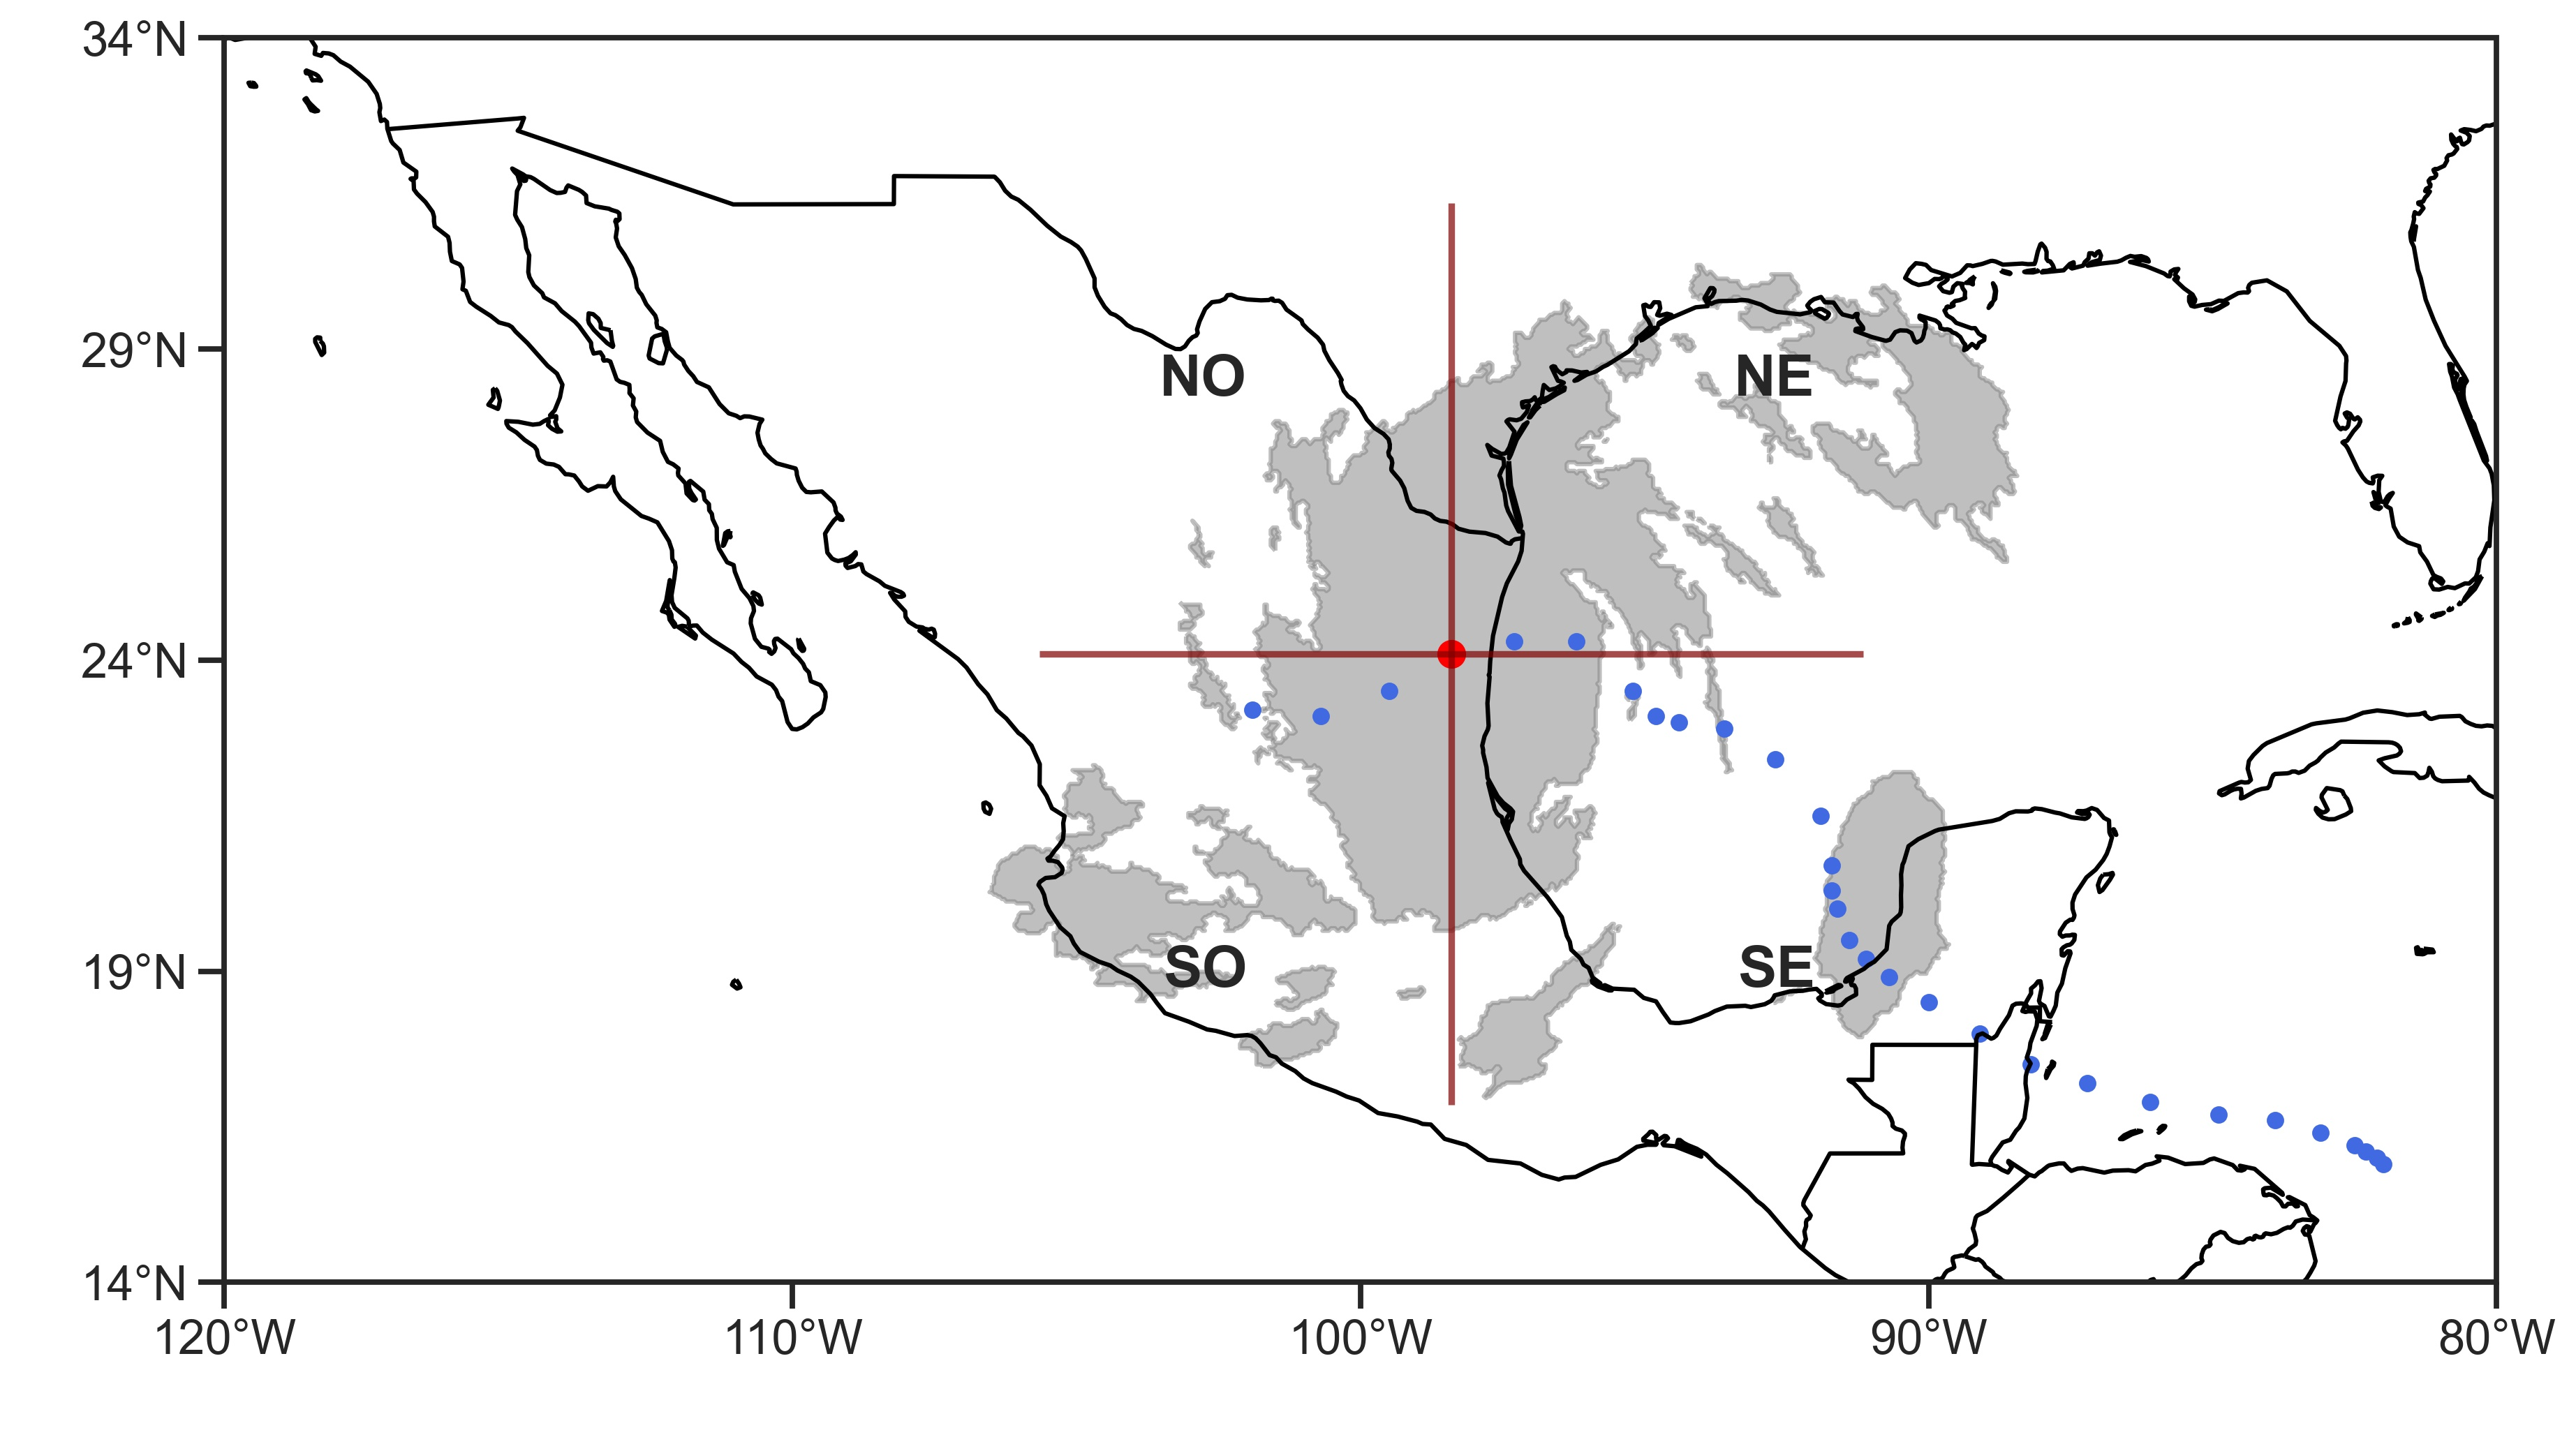
\includegraphics[scale = 0.32]{Images/Figures/Fig_2_3.jpeg}
        \caption{Extensión del campo de nubes a través de contornos generados con imágenes IR (contornos grises) del huracán Alex 2010, cuyas posiciones están representadas por puntos azules}
        \label{fig:fig_5}
    \end{figure}
\end{frame}

\subsection{Métodos para relacionar la lluvia con el tamaño del ciclón}
\begin{frame}
\begin{enumerate}
\setcounter{enumi}{0}
\item Algoritmo del Radio de las Bandas de Precipitación
(RBP)
      \begin{figure}
            \centering
            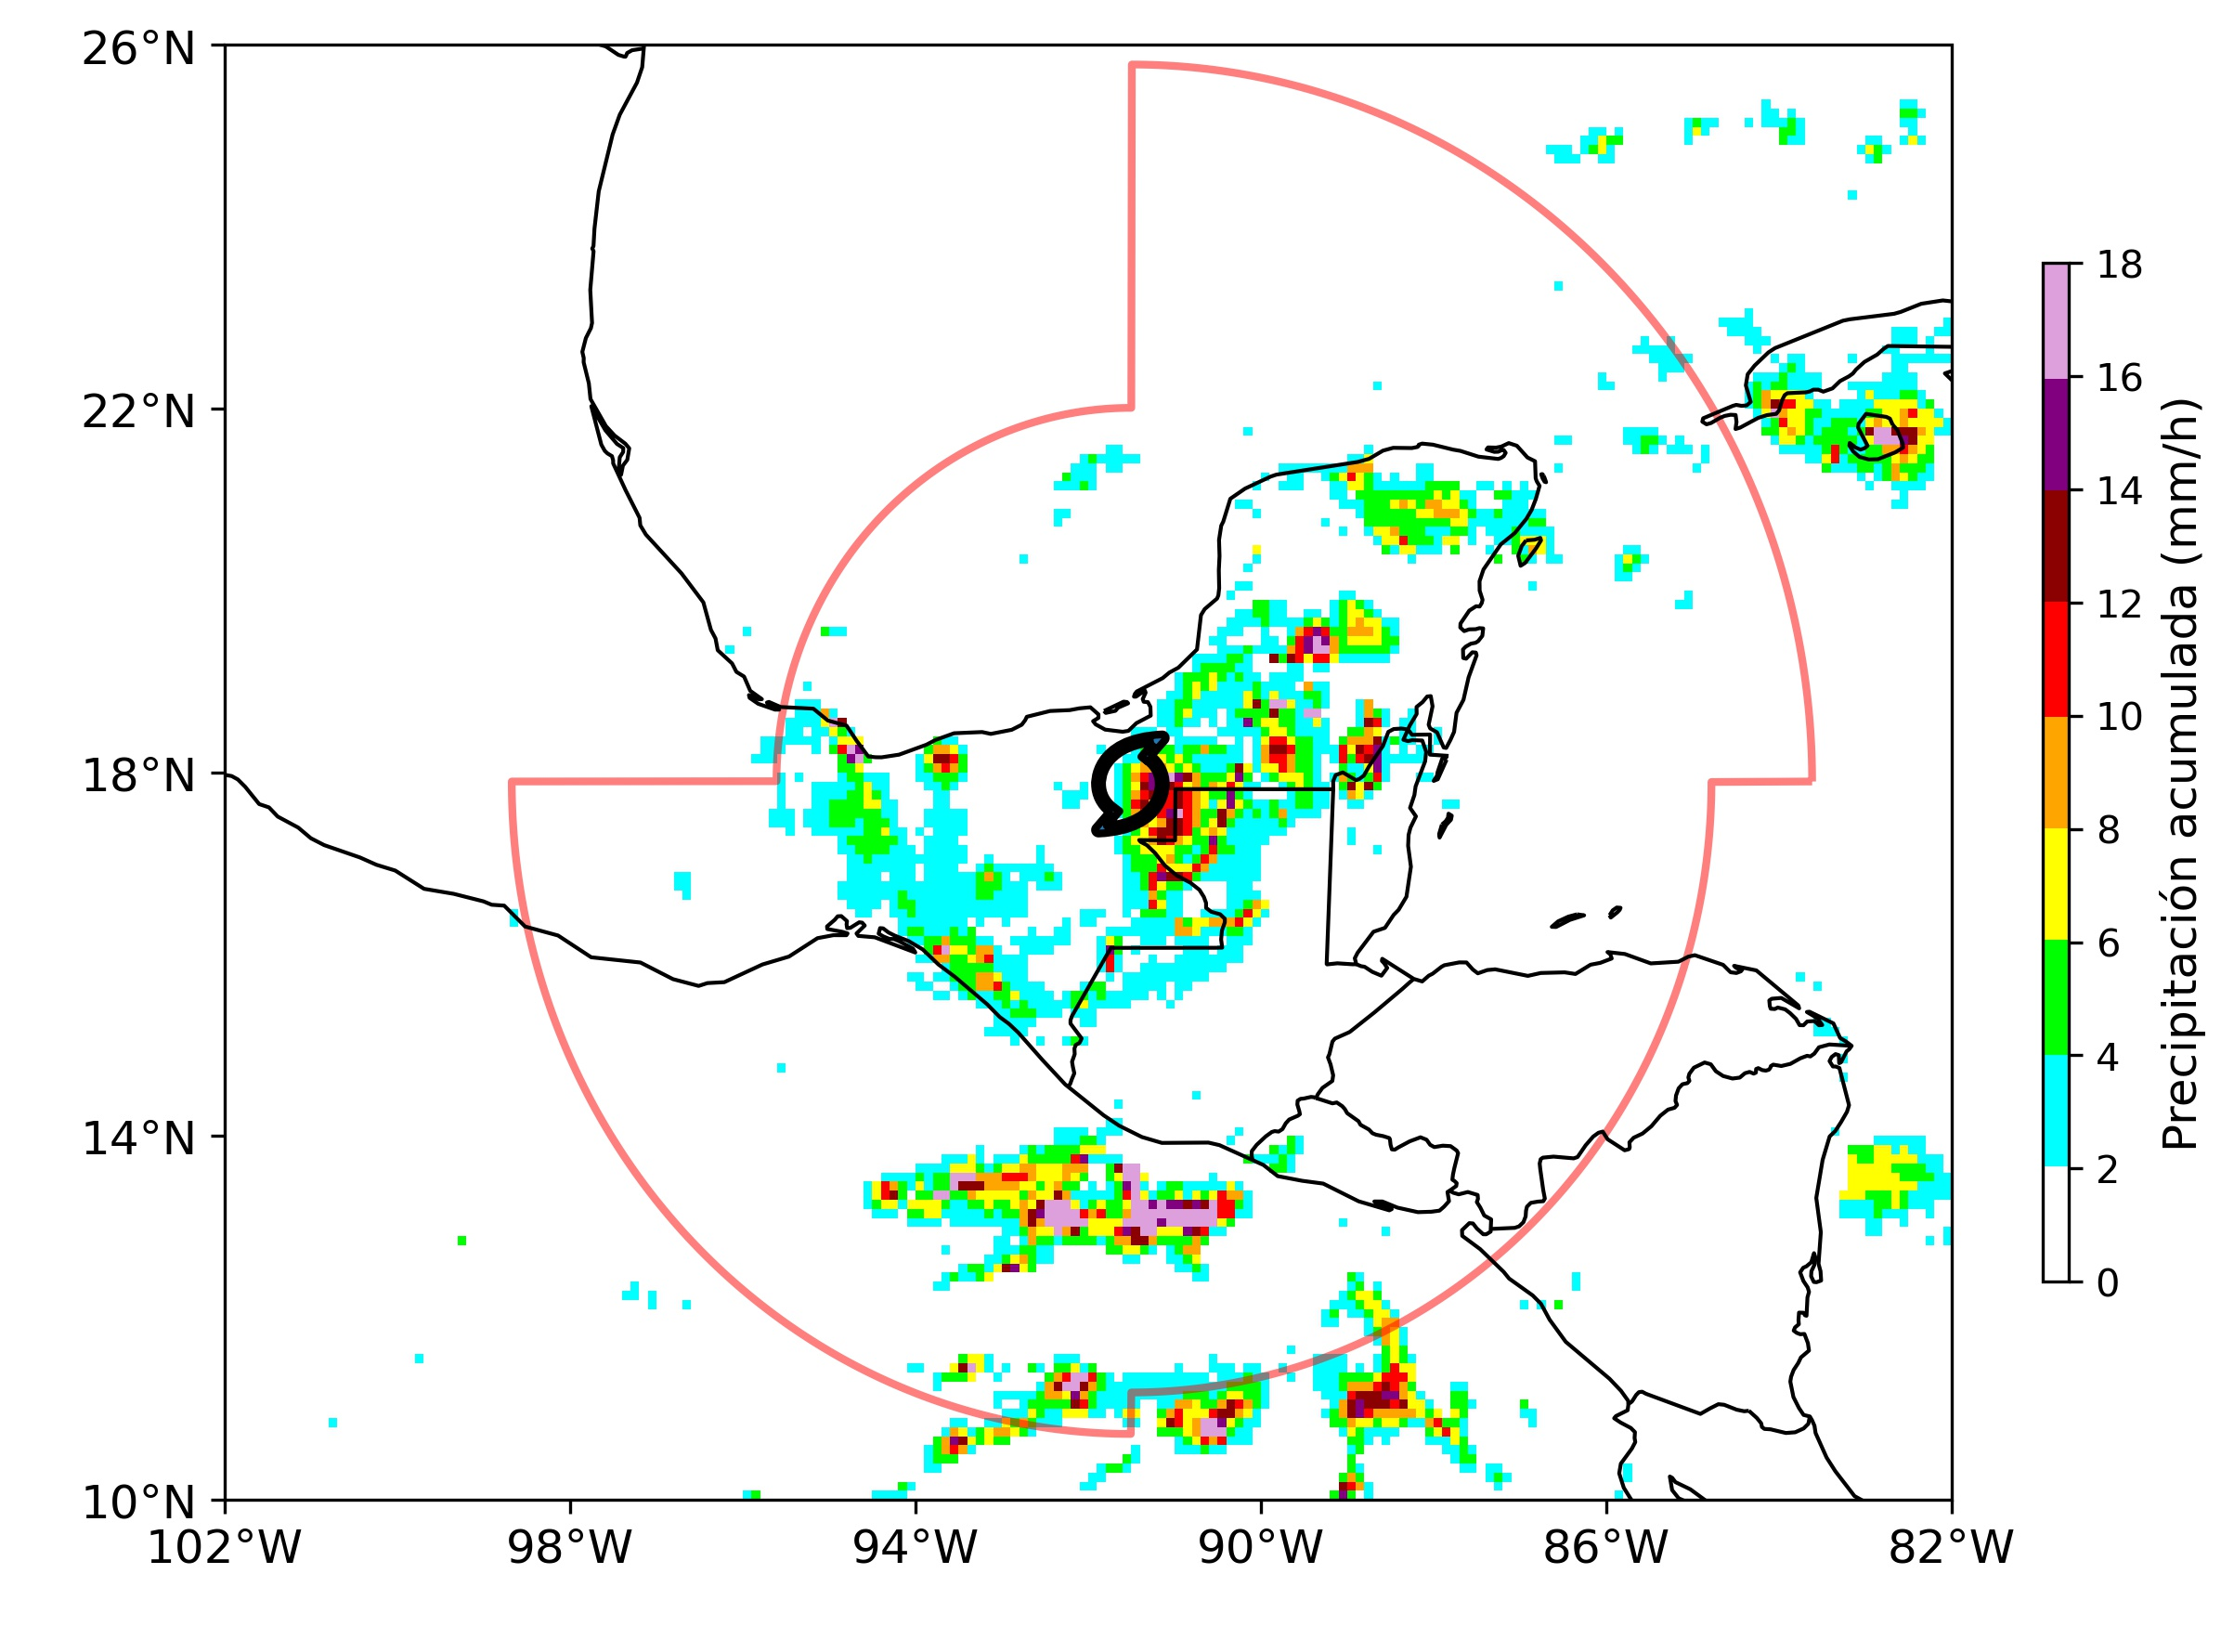
\includegraphics[scale = 0.39]{Images/Figures/Fig_2_5.jpeg}
            \caption{Valores de precipitación del GPM\_IMERG para la TT Cristóbal en su posición del 4 de junio del 2020 a las 06:00 UTC.}
            \label{fig:fig_6}
        \end{figure}
\end{enumerate}
\end{frame}

\begin{frame}
\begin{enumerate}
\setcounter{enumi}{1}
\item Técnica de anillos usando los datos de GPM\_IMERG
      \begin{figure}
            \centering
            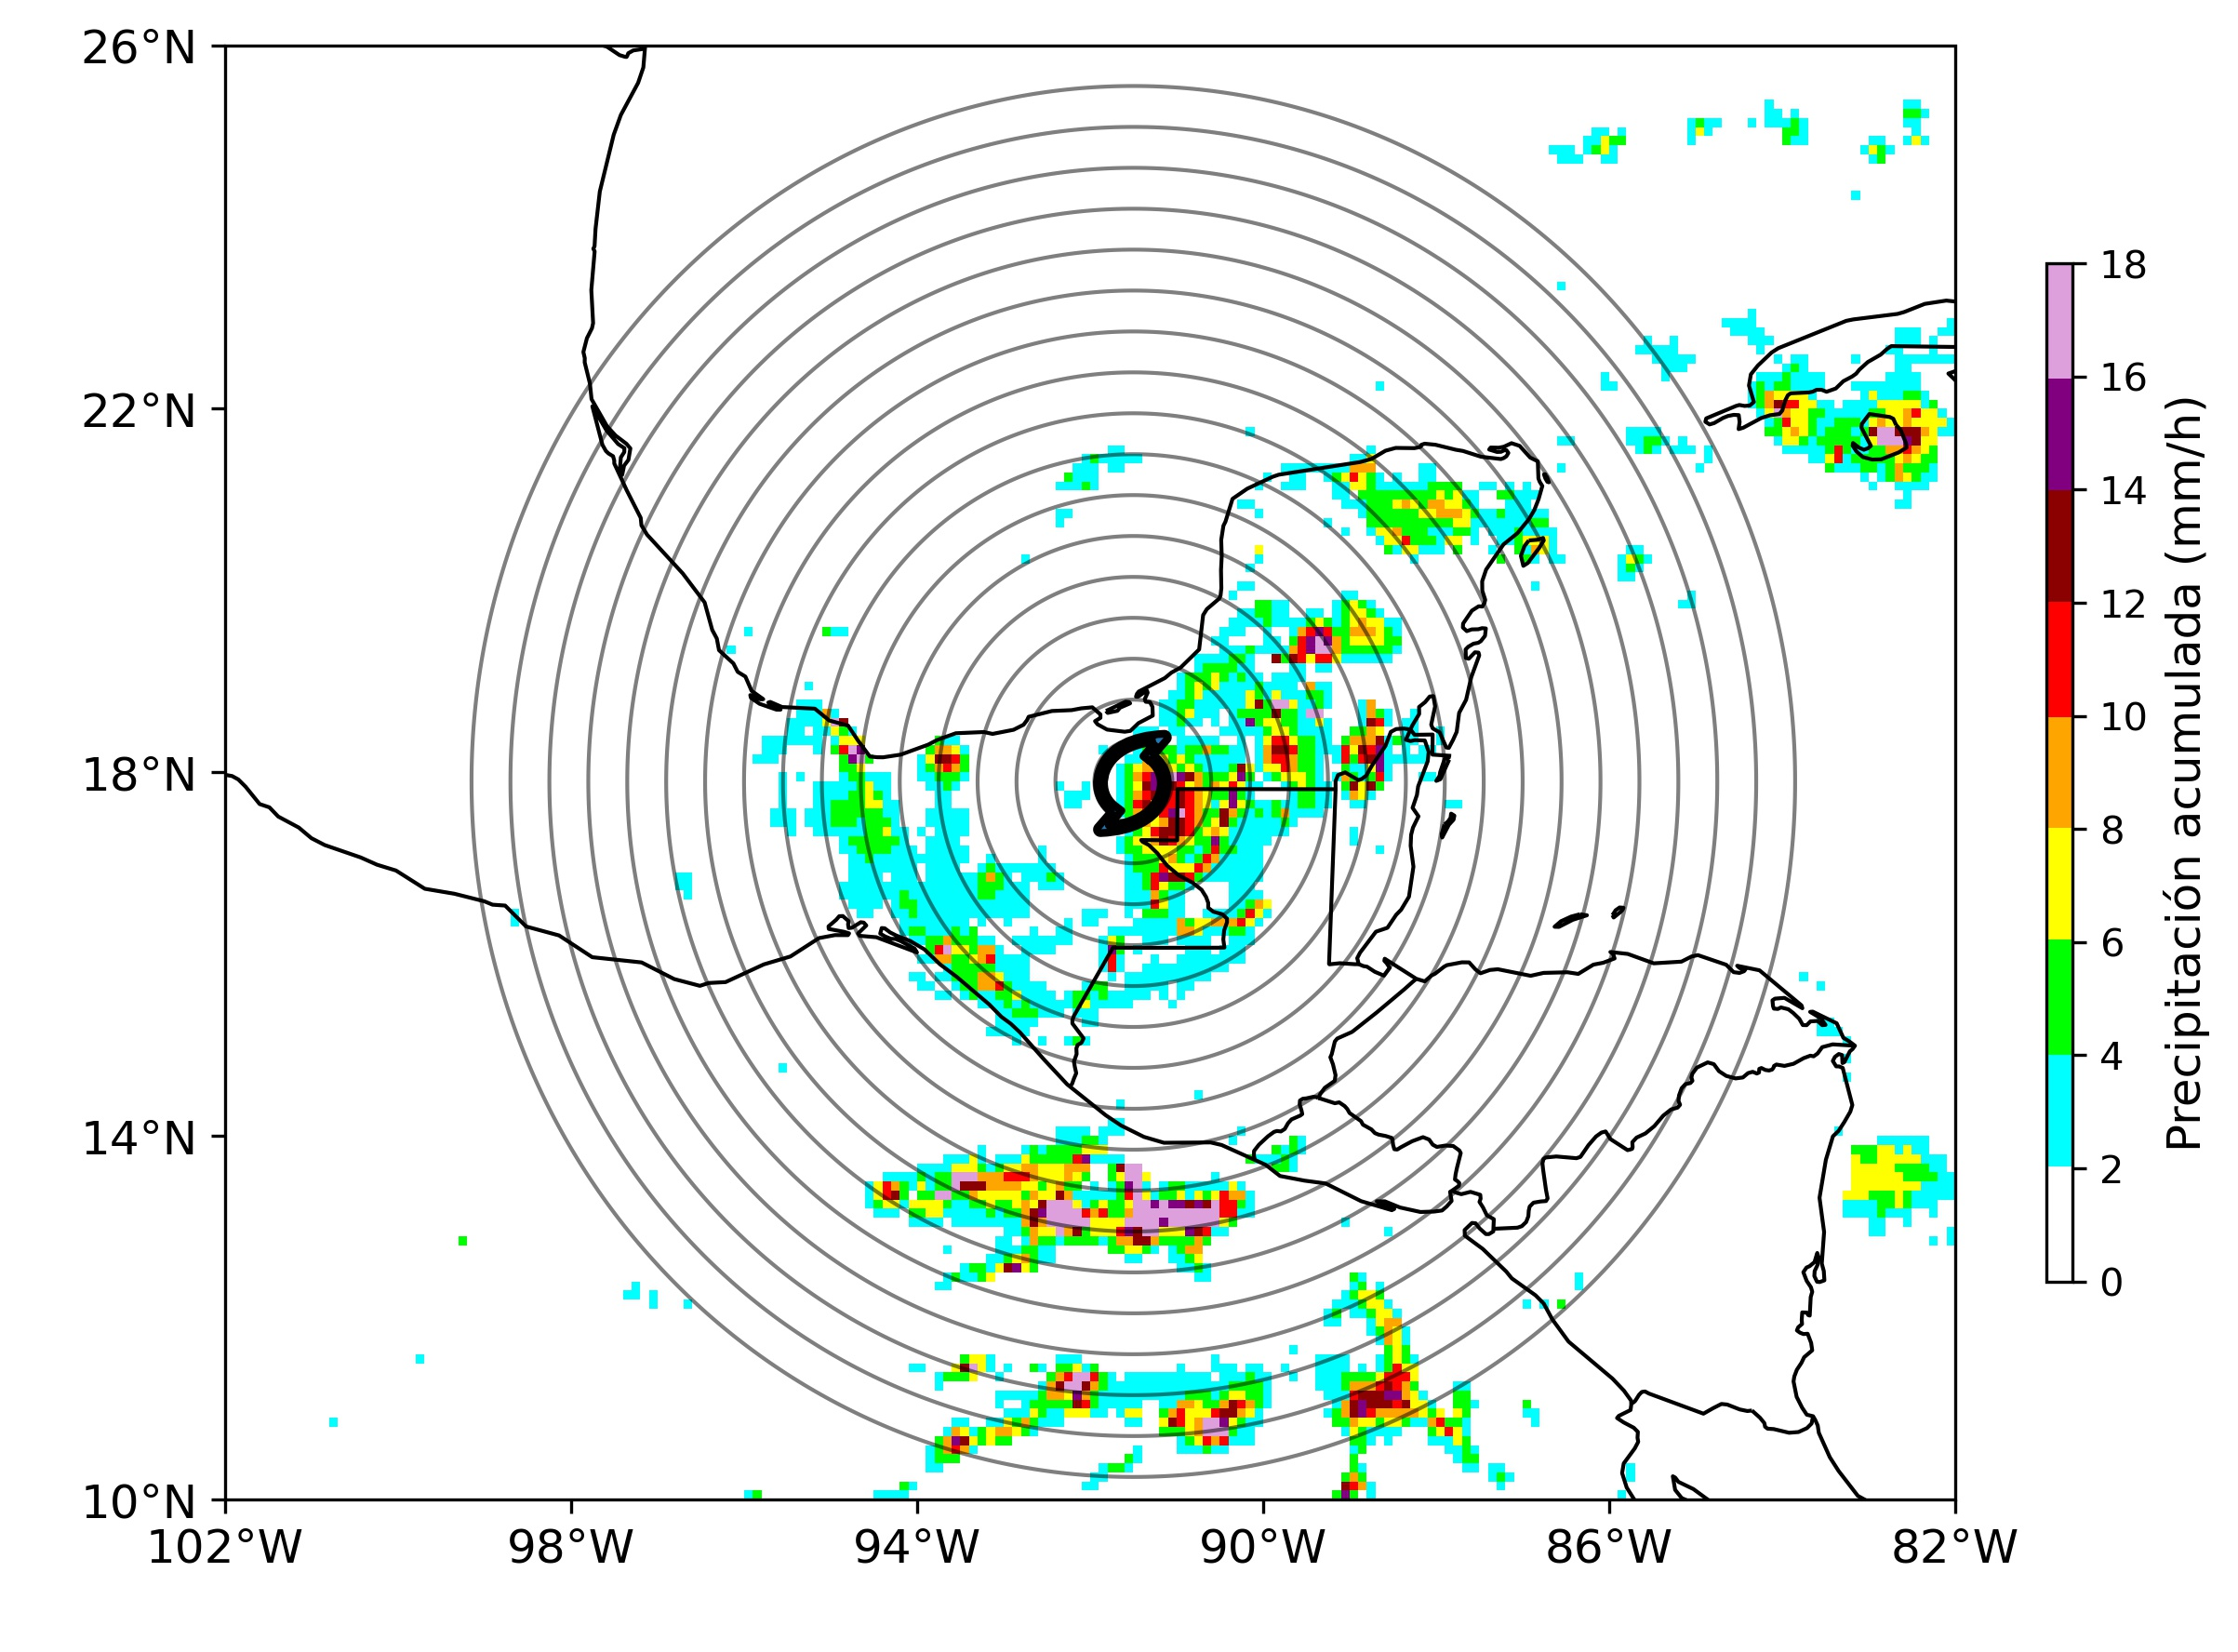
\includegraphics[scale = 0.4]{Images/Figures/Fig_2_6.jpeg}
            \caption{Similar a la Fig. \ref{fig:fig_6}, pero mostrando los anillos usados cada 50 km.}
            \label{fig:fig_7}
        \end{figure}
\end{enumerate}
\end{frame}

\begin{frame}
\begin{enumerate}
\setcounter{enumi}{2}
\item Técnica de anillos usando los datos continentales de CHIRPS
      \begin{figure}
            \centering
            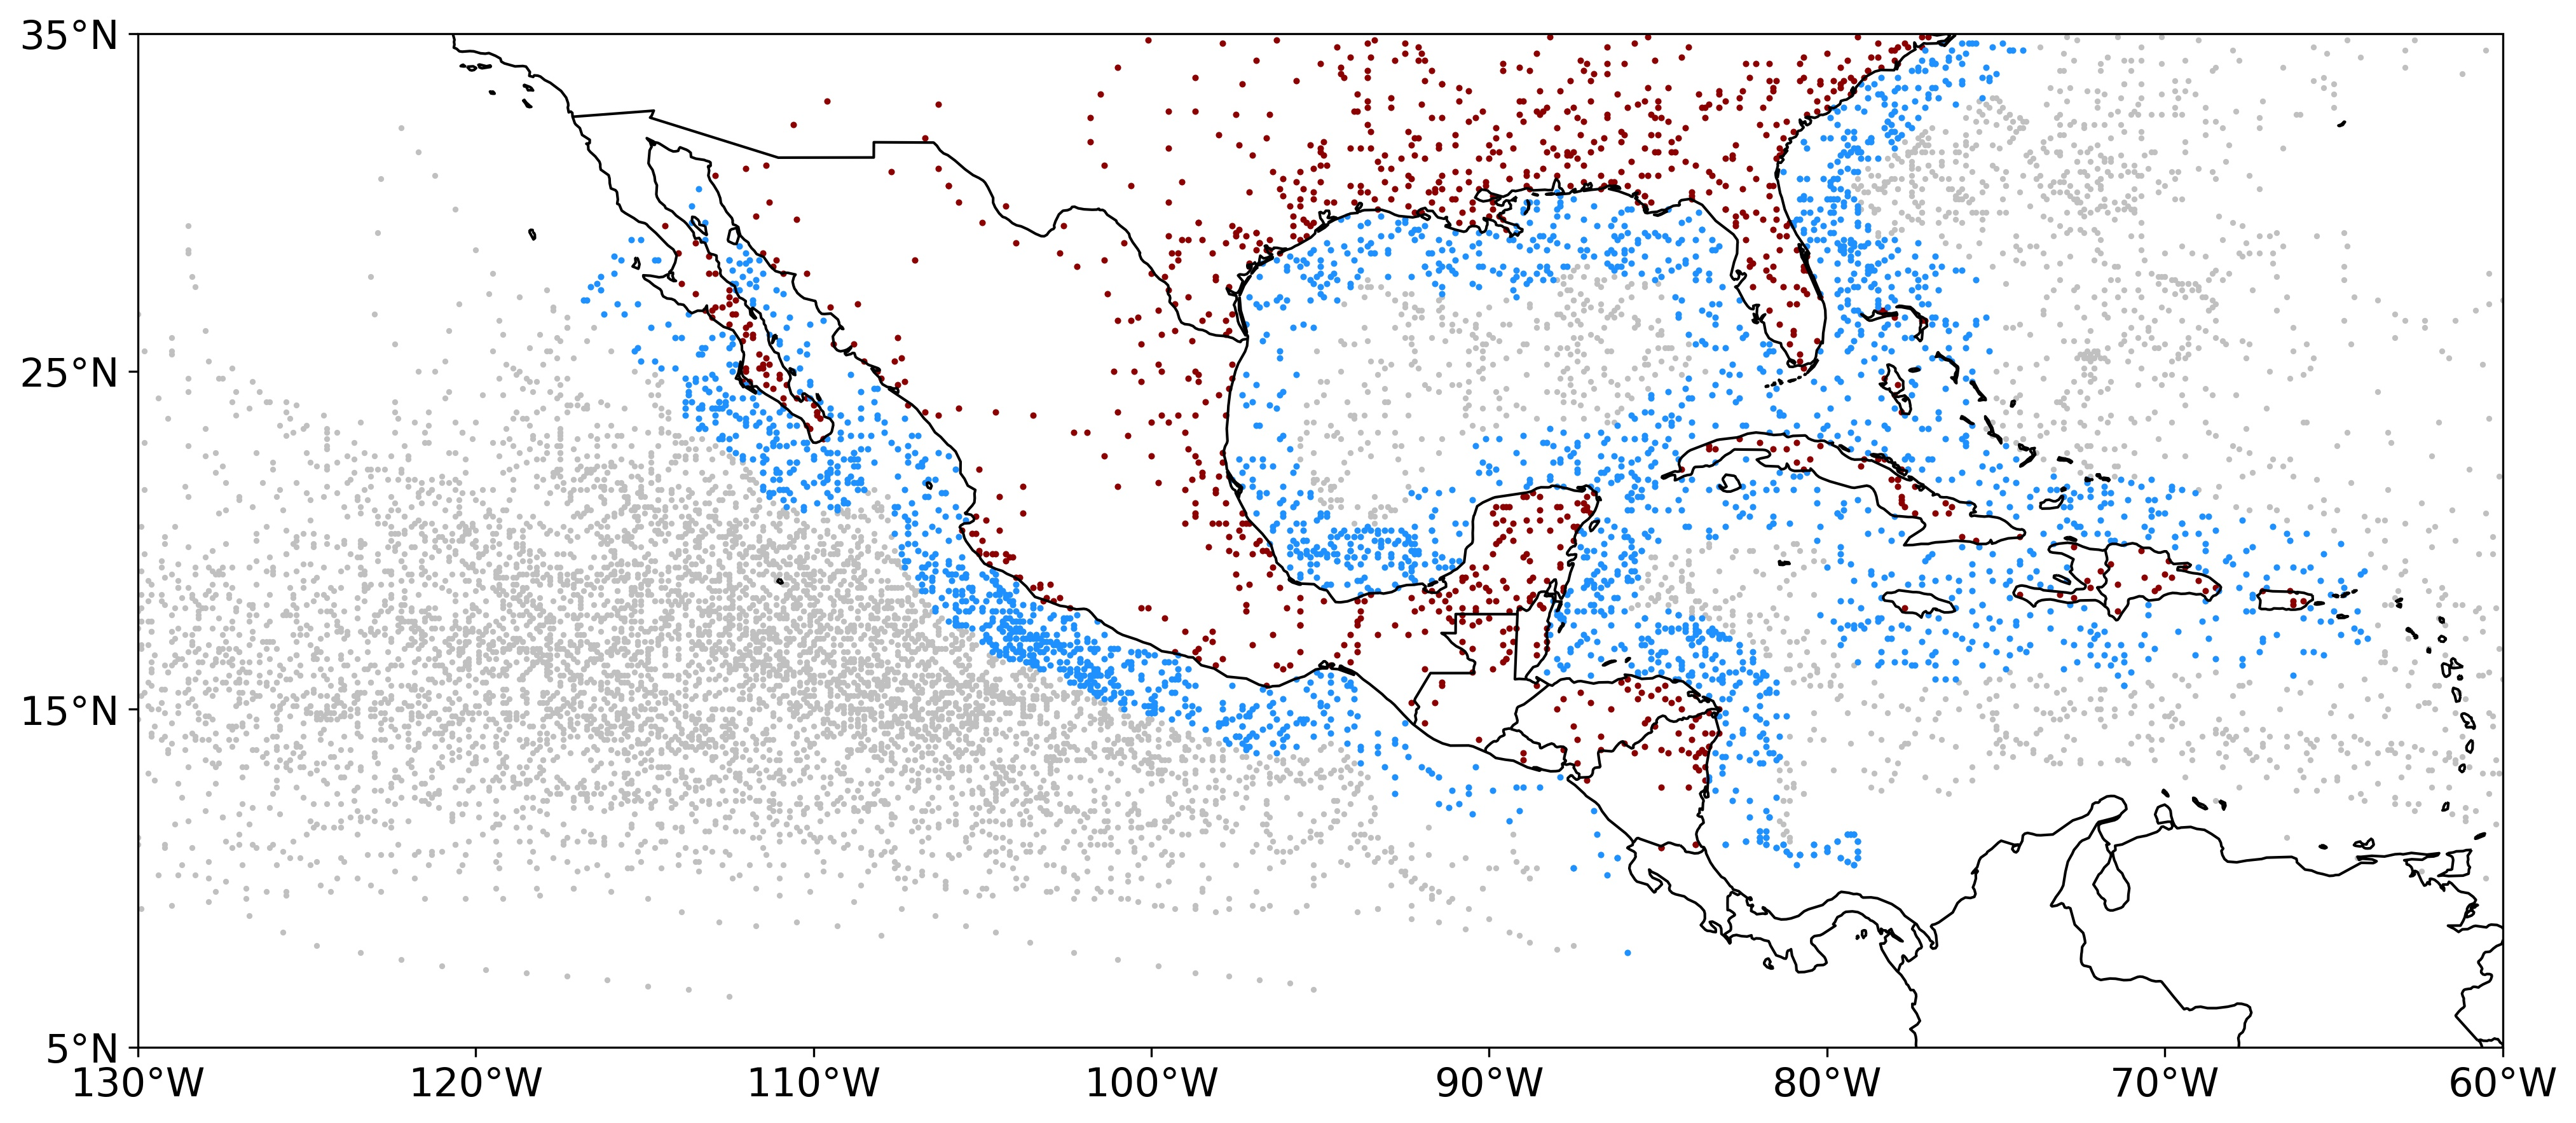
\includegraphics[scale = 0.24]{Images/Figures/Fig_2_7.jpeg}
            \caption{Posiciones de los CT que se encuentran sobre territorio mexicano (rojo) y cercanos a la costa (distancia a 250 km, en azul).}
            \label{fig:fig_8}
        \end{figure}
\end{enumerate}
\end{frame}

\subsection{Sobre las variables medioambientales y la forma}

\begin{frame}
    \begin{alertblock}{Relaciones estadísticas}
        \begin{enumerate}
            \item Correlación Spearman
            \item Modelos de Estimación de Ecuaciones Generalizadas
        \end{enumerate}
        ~\
    \end{alertblock}
~\
    
    \begin{exampleblock}{La forma del CT}
        \begin{enumerate}
            \item Dispersión
            \item Asimetría
            \item Solídez
        \end{enumerate} 
        ~\
    \end{exampleblock}
\end{frame}

\section{Resultados}

\subsection{Sobre la climatología del tamaño de los CTs}
\begin{frame}
\begin{itemize}
    \item Se analizaron {\red 191} y {\gray 337} CTs de las cuencas {\red NA} y {\gray EP} respectivamente durante el periodo 2000-2020.
    \\~\
    \item Sólo se consideran las posiciones de CT de 6 horas que se localizan en la región de estudio. Se obtuvieron {\red 4526} y {\gray 6923} posiciones de CTs para las cuencas.
\end{itemize}
\end{frame}

\begin{frame}
    \begin{figure}
        \centering
        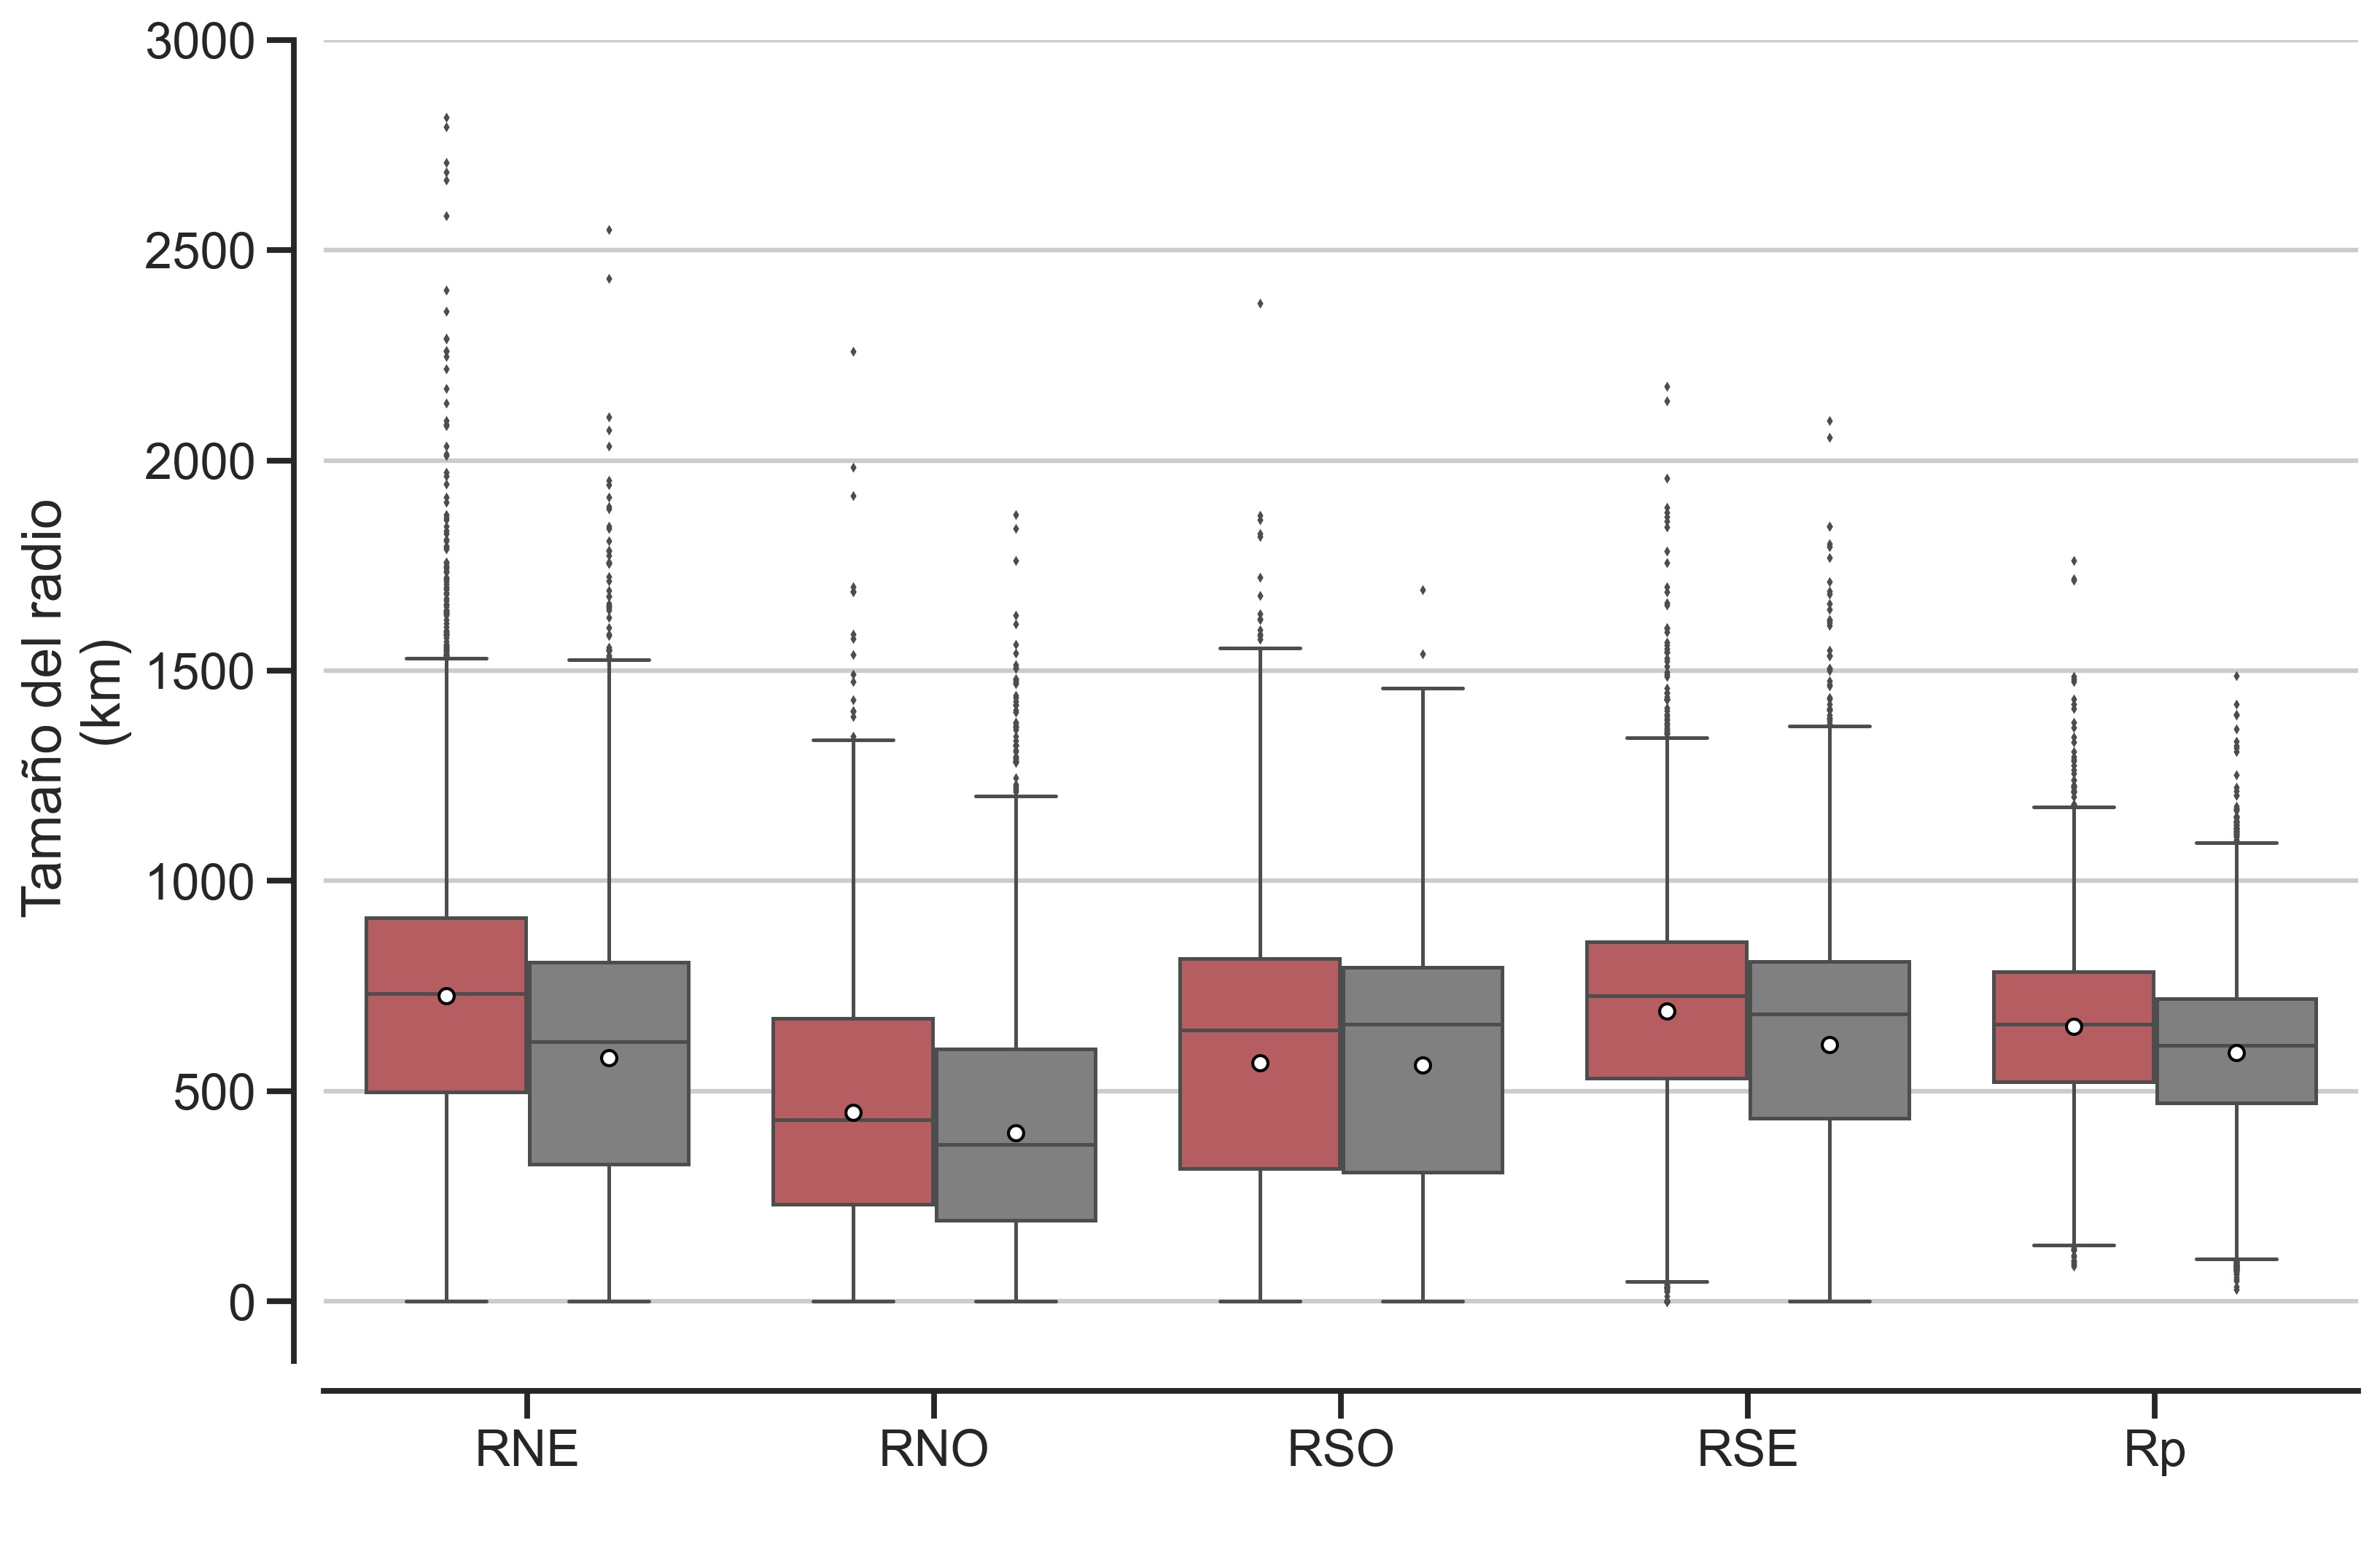
\includegraphics[scale = 0.35]{Images/Figures/Fig_3_1.jpeg}
        \caption{Cajas y bigotes de las distribuciones de los radios por cuadrante y el $R_p$ (km) de los radios en la región de estudio de la cuenca {\red NA} y {\gray EP}.}
        \label{fig:fig_9}
    \end{figure}
\end{frame}

\subsection{Sobre la relación del tamaño y la precipitación}
\begin{frame}

\end{frame}

\subsection{Sobre las variables medioambientales y la precipitación}
\begin{frame}
\begin{itemize}
    \item Algunos CT muestran una fuerte divergencia en la atmósfera superior. Puede estar relacionado con grandes cantidades de humedad en la atmósfera de nivel medio, lo que produce tasas de precipitación intensas de CT en la superficie.

    \item Los CTs en ambientes secos producen menos precipitación y tienen menores extensiones radiales de viento en comparación con los CTs en ambientes húmedos.

    \item La cizalladura del viento es más importante para los CT sobre la cuenca de {\red NA}. Esto último está posiblemente relacionado con el hecho de que las trayectorias de los CT cerca de la masa continental son modificadas por la cizalladura ambiental.

    \item Ni la intensidad del CT ni la presión central a nivel del mar son importantes para la estimación de la precipitación del CT, situado dentro del tamaño exterior del CT.
\end{itemize}
\end{frame}

\subsection{Sobre la forma del CT}
\begin{frame}
\begin{figure}
    \centering
    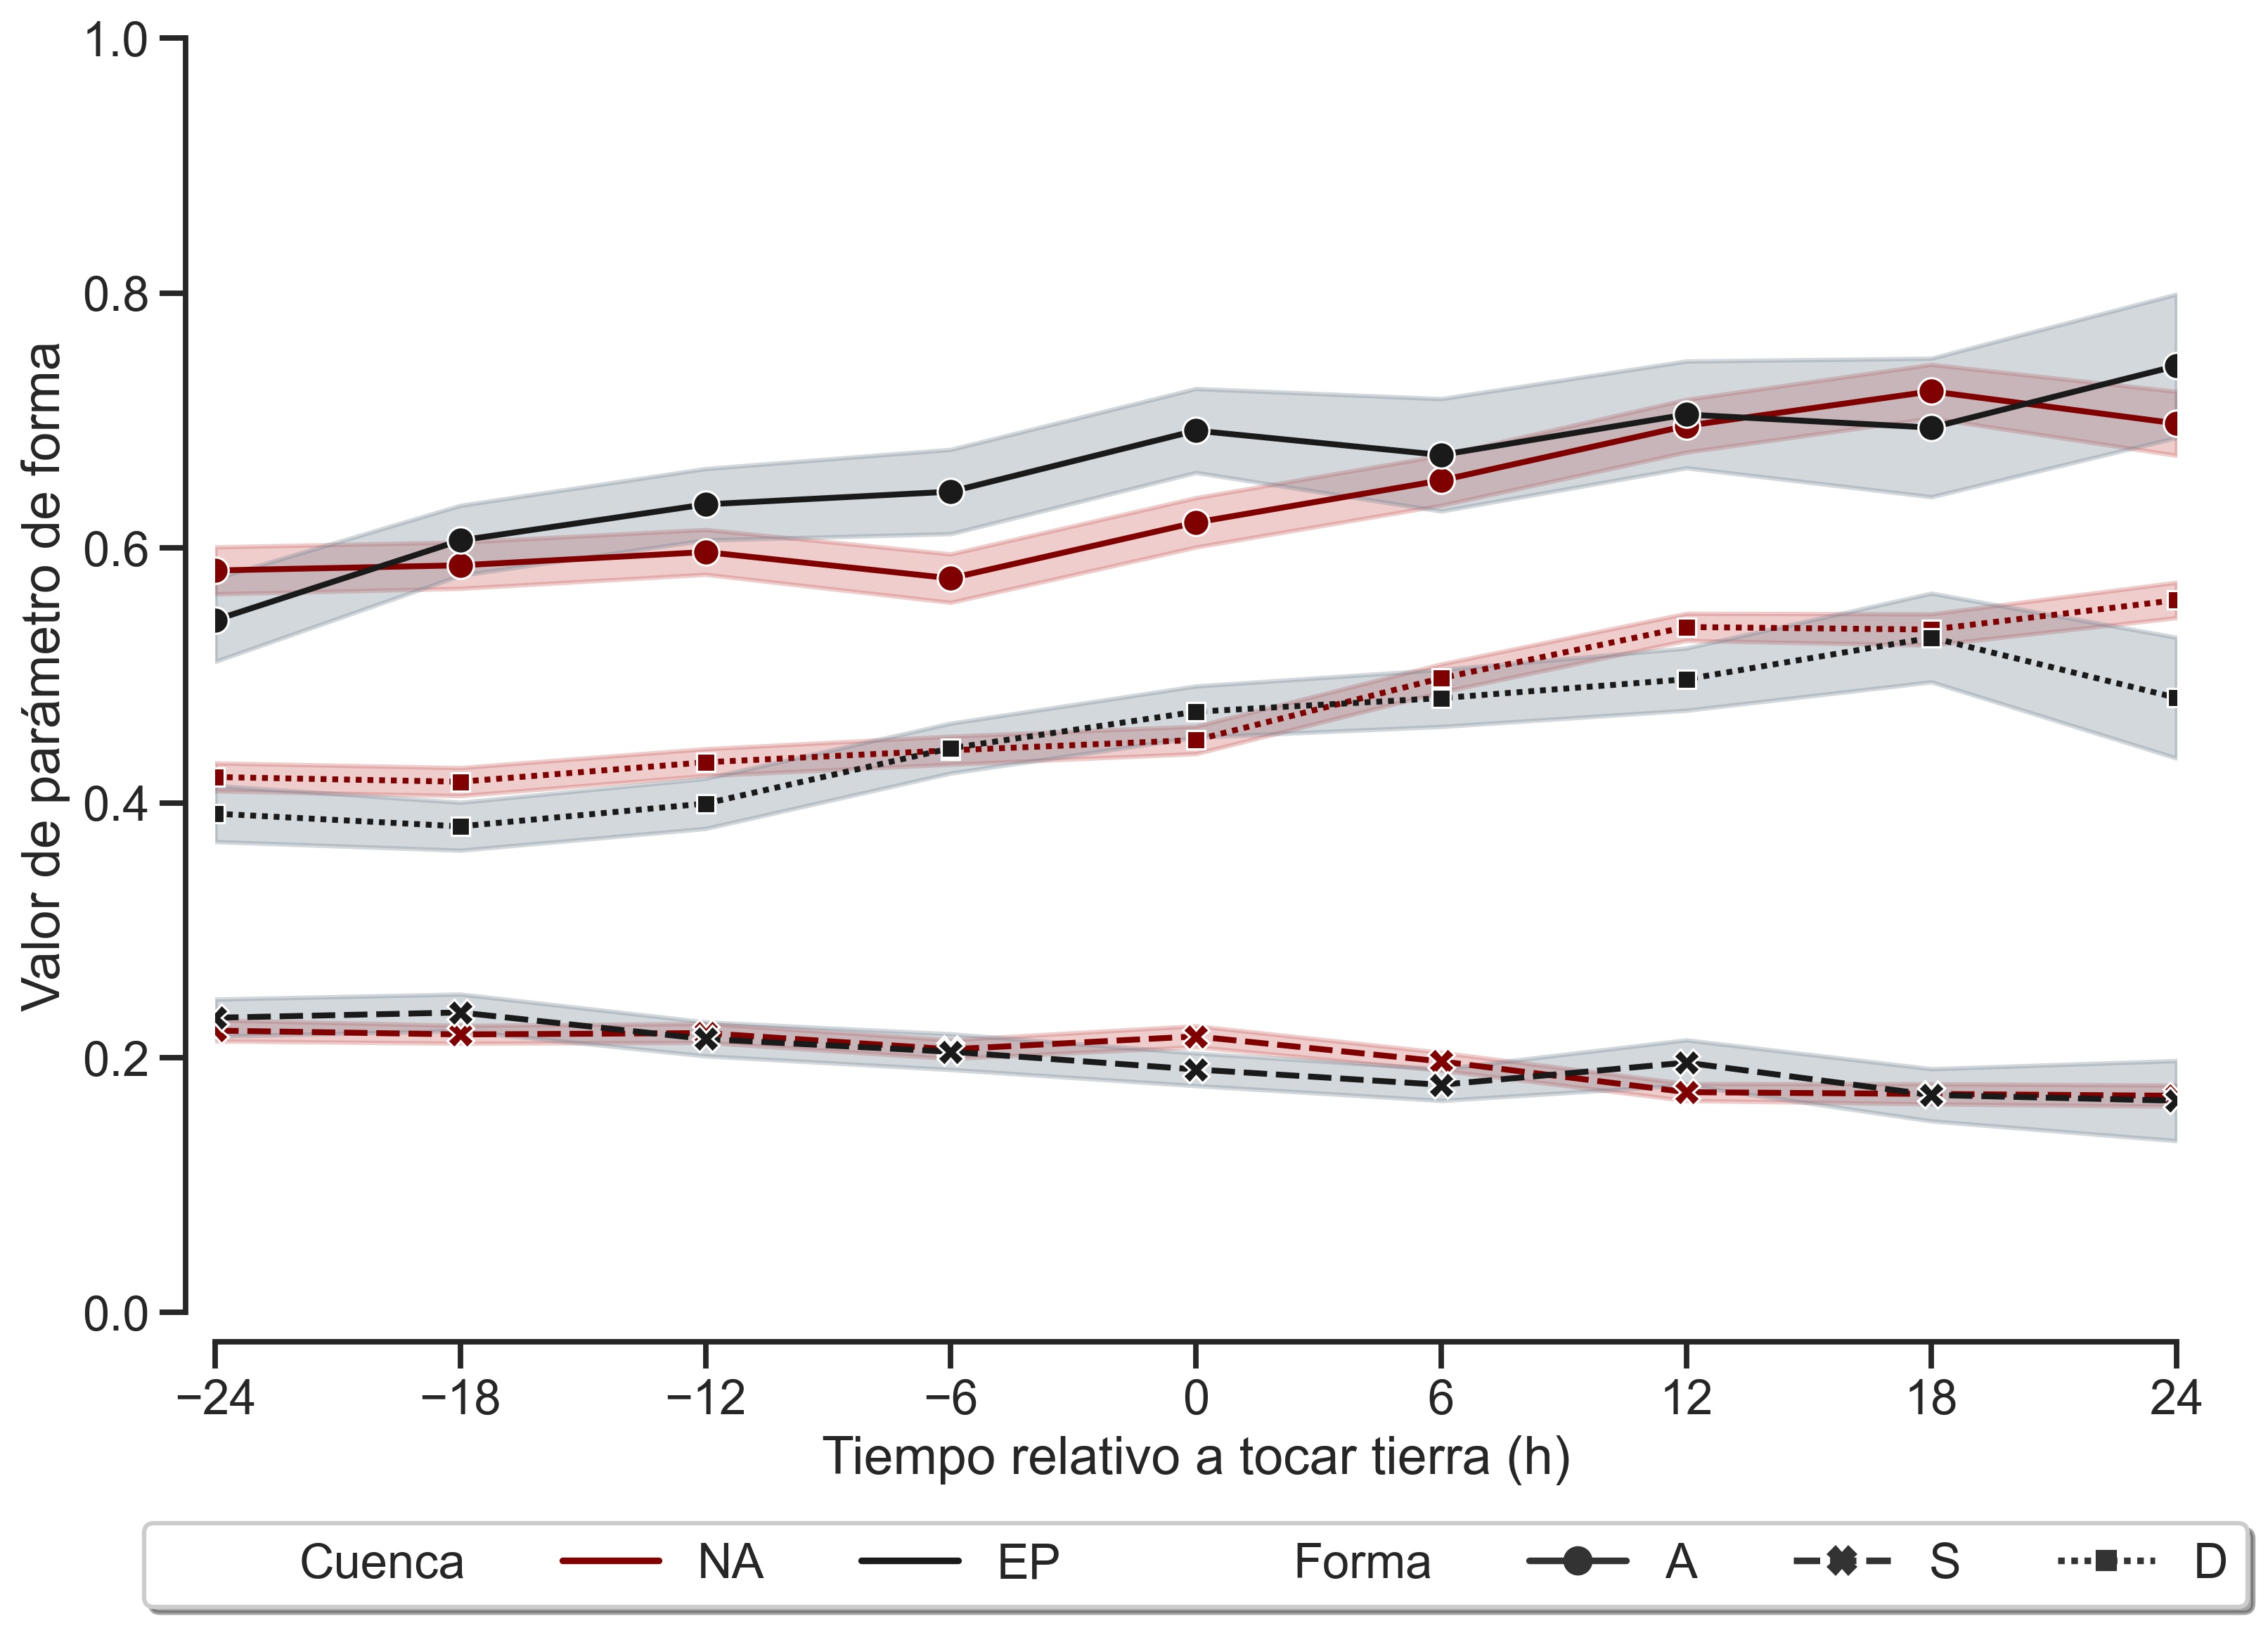
\includegraphics[scale = 0.3]{Images/Figures/Fig_3_32.jpeg}
    \caption{Comportamiento promedio de las métricas de forma de los CTs de la cuenca {\red NA} y {\gray EP}, 24h antes (-24) y 24h después (24) de hacer \textit{landfalling}.}
    \label{fig:fig_10}
\end{figure}
\end{frame}
\section{Conclusiones y Trabajo Futuro}
\begin{frame}{Conclusiones}
    \begin{enumerate}
        \item<1-> El tamaño del CT calculado con el algoritmo ROCLOUD muestra ser operacionalmente funcional. Otros estudios similares no tienen en cuenta la precipitación del CT. 
        \\~\
        \item<2-> Además, la intensidad del CT no está relacionada con su tamaño. Por ejemplo, los TD pueden tener un tamaño mayor que los huracanes.
        \\~\
        \item<3-> La precipitación del CT calculada a partir de dos enfoques (radio de las bandas de lluvia del CT y perfiles pcp) muestra que los CT producen importantes precipitaciones en regiones remotas situadas a ~750 km del centro del CT. Es  mayor sobre las regiones continentales ya que las bandas de lluvia están más dispersas que sobre las regiones oceánicas.
    \end{enumerate}
\end{frame}

\begin{frame}{Conclusiones}
    \begin{enumerate}
    \setcounter{enumi}{3}
        \item<1->Las variables a gran escala desempeñan un papel importante en la determinación de las precipitaciones del CT.
        \\~\
        \item<2->La humedad a niveles medios, la cizalladura del viento y la divergencia en la atmósfera superior muestran una fuerte relación con la precipitación del CT. 
        \\~\
        \item<3->Finalmente, las métricas de forma Dispersión ($D$), Asimetría ($A$) y Solidez ($S$) muestran que, en promedio, los CTs de ambas cuencas tienden a ser más dispersos, asimétricos y menos sólidos.
    \end{enumerate}
\end{frame}

\begin{frame}
\begin{columns}
    \begin{column}{0.5\textwidth}
        \begin{block}{\textbf{Sobre el SIAT-CT}}
        La motivación principal de este trabajo radica en las limitaciones que tiene el SIAT-CT en términos de la definición del tamaño. Los resultados muestran que la influencia de la PCT puede alcanzar los 750 km desde el centro del CT. Por ello, se vuelve relevante usar una definición diferente al R34, que incorpore un tamaño del CT que considere la extensión de las bandas nubosas del CT y su precipitación.
        \end{block}
    \end{column}
    \begin{column}{0.5\textwidth}
    \begin{figure}
        \centering
        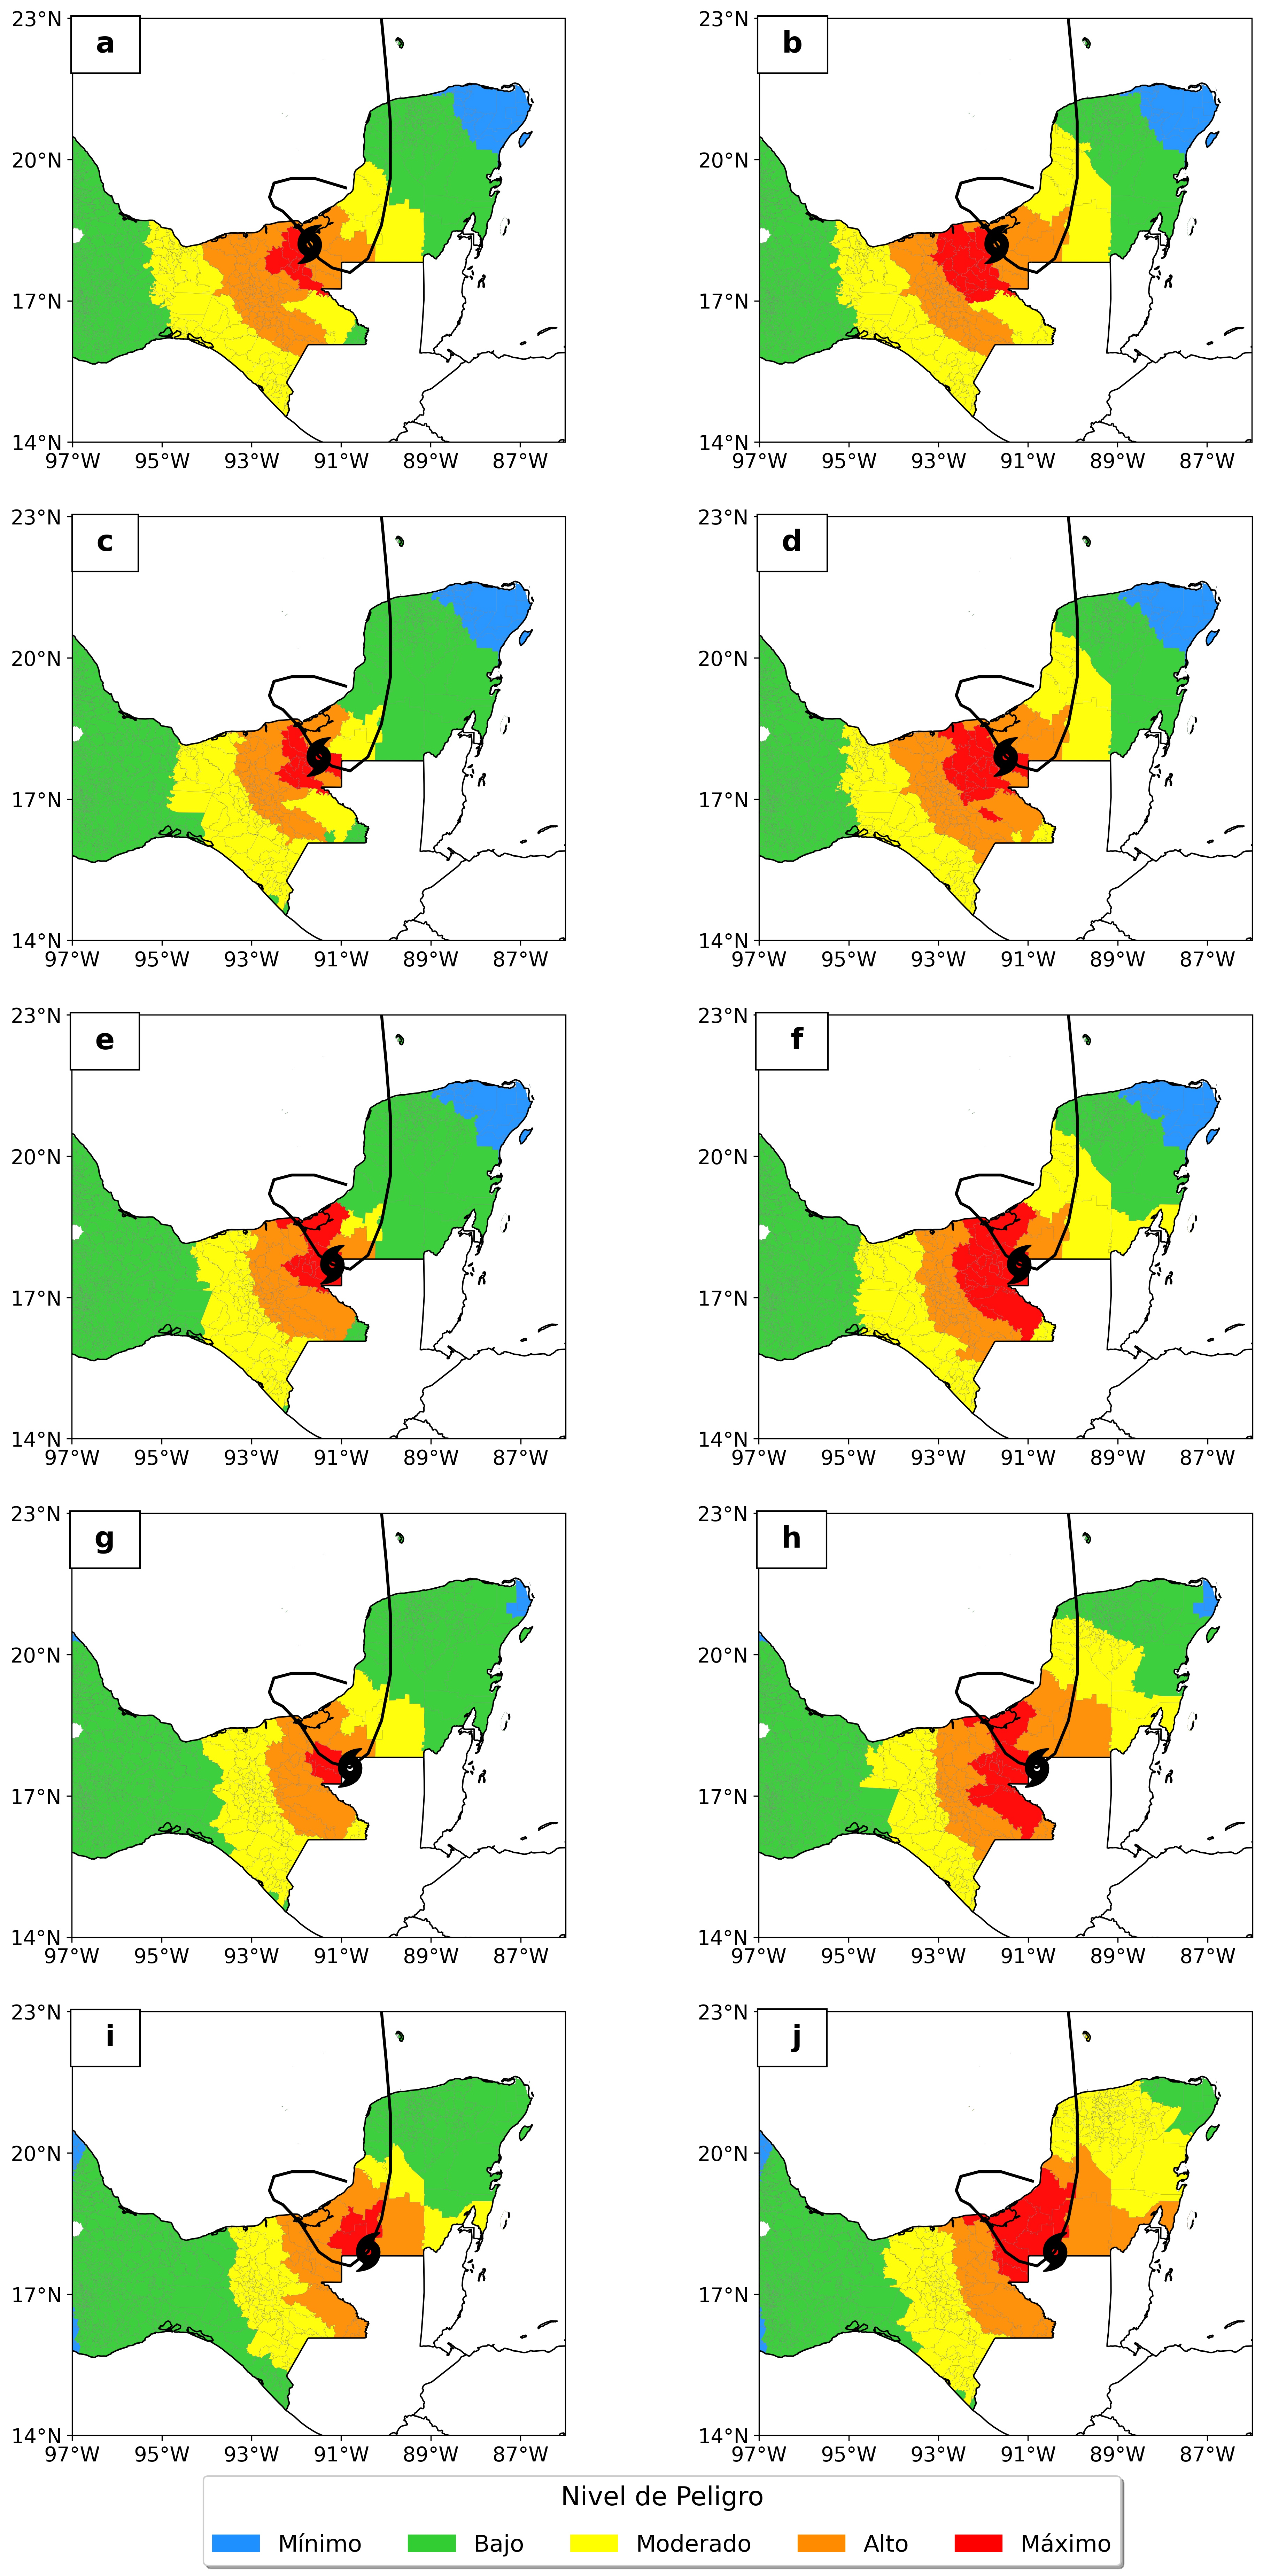
\includegraphics[scale = 0.135]{Images/Figures/Fig_4_1.jpeg}
        \label{fig:fig_conclusion}
    \end{figure}
    \end{column}
\end{columns}
\end{frame}

\begin{frame}{Trabajo Futuro}
    \begin{itemize}
        \item Estudiar posibles mejoras en las alertas tempranas modificando los tamaños del CT.
        \\~\
        \item Usar técnicas de machine learning para predecir el tamaño de un CT, con fines operativos.
        \\~\
        \item Estudiar el cambio climático y su papel en el tamaño de los CTs en un futuro.
    \end{itemize}
\end{frame}


% This section is a placeholder for you to go over crucial points to takeaway from your presentation.

\begin{frame}
\begin{center}
\Huge ¡Muchas Gracias!
\end{center}
\end{frame}

% Bibliography/References
%\begin{frame}[allowframebreaks]
%	\frametitle{References}
%	\nocite{*}
%	\printbibliography
%\end{frame}

\end{document}